
\section{Major points}

\subsection*{Reviewer comment 1}

A major aspect of the study concerns the representation of the particle size
distribution which is retrieved by two free parameters (different from the 2
moments of the atmospheric model GEM used to provide the test scenes) and the
assumptions of the particle type. The difficulty of connecting atmospheric model
output to single scattering properties (which is one of the fundamental
assumptions) could be better explained. The motivation why the authors choose
their approach and why they test certain settings need to be discussed in the
beginning. Couldn’t Tab. 1 and 4 be combined and better explained which is used
for which purpose? Why is cloud ice the same and GEMsnow and GEMGraupel different
in both?

\subsubsection*{Author response}

We agree with the comment that the rather arbitrary choice of tested particles
is a weak spot of the study. To improve this, the experiments will be repeated
with a more principled selection of particles. The new selection is based on the
particle properties described in \citet{ekelund20} and covers a broader range of
mass-size relationships and scattering parameters. In particular, the GemSnow
model has been removed from the selection of test particles because it does not
cover small ice particle sizes.


\subsubsection{Changes in manuscript}

\begin{itemize}
\item A paragraph has been added to the description of the GEM test scenes which explains
  the particle models that have been developed to match the assumptions of
  the GEM microphysics scheme and that are used to simulate observations.

  \begin{change}[110]
  \DIFadd{In order to simulate observations from the GEM model scenes, the hydrometeor
  classes of the GEM microphysics scheme must be associated with particle shapes
  to define their radiometric properties. The ARTS single-scattering database,
  described in more detail below, contains particle models which were designed to
  be consistent with the mass-size relationships assumed in the GEM model. The
  particle shapes used to represent the GEM model's different hydrometeor types
  are listed together with their properties in
  Tab.~1.
  }\DIFaddend 
  \end{change}

\item The following has been added to the description of the retrieval
  implementation which discusses the difficulty of representing the complex
  mixture of different particles in the GEM model scenes with a single particle
  model as well as the new selection of particle models and habit mixes.

  \begin{change}[231]

\DIFadd{A major difficulty for cloud retrievals is that the observations may not provide
sufficient information to distinguish different hydrometeor species. Due to this
ambiguity, frozen hydrometeors in the proposed retrieval algorithm are
represented using only a single hydrometeor species. It is therefore necessary
to find a suitable representation for frozen hydrometeors, which can capture the
variability of the four frozen hydrometeor species in the GEM model and ideally also
that of real ice hydrometeors.
}

\DIFadd{The differences between hydrometeor species in the test scenes are due
  to their different concentrations, sizes and shapes (c.f. Fig.~2). Since two
  parameters of the PSD of frozen hydrometeor species are retrieved, the
  retrieval is able to represent the characteristic number concentrations and
  particle sizes of different hydrometeor species. Variations in particle shape
  which correlate with particle size can be represented using a habit mix
  combining crystal shapes at small sizes with aggregates or rimed particles at
  larger sizes. This provides the retrieval with some flexibility to represent
  the different shapes present in the test scenes. }

\DIFadd{Even with this configuration the simplified retrieval forward model will not be
able to represent every possible configuration of mixes of the four ice
hydrometeor species in the GEM model. It thus remains unclear which particle
shape should be used to best represent this mixture. We therefore choose a set
consisting of multiple particle shapes and habit mixes, which will be used in
the retrieval to study the impact of the choice of the particle shape on the
retrieval results. The selected particles are listed in
Tab.~4. Three of them, GEM Cloud Ice, GEM Snow, and
GEM Graupel, correspond to the shapes present in the GEM model scenes. The GEM
Snow and Graupel habits were mixed with crystal shapes to ensure that they cover
sizes down to around $10\ \unit{\mu m}$. In addition to this, two of the habit
mixes distributed with the ARTS SSDB, the Large Plate Aggregate and Large Column
Aggregate standard habits, are included in the selection to increase the range of
scattering properties it covers.}\DIFaddend
  \end{change}

\item The errors in the reported parameters of the mass-size
  relationship for the GEM Snow and GEM graupel particles have been
  corrected.
\end{itemize}

It was, however, not possible  to combined Tab.~1 and Tab.~4
because they convey slightly different information.

%The following changes will be introduced in the manuscript:
%
%\begin{itemize}
%\item To explain how hydrometeor concentration from the model scenes are
%  connected to ice particle models  the following paragraph will be added
%  to sections describing the GEM model scenes:
%
%  \begin{change}[101]
%\DIFaddbegin \DIFadd{In order to simulate microwave observations for the GEM model scenes, the
%hydrometeor classes in the model must be associated with particle models that
%define their shape and thus their radiometric properties. The ARTS
%single-scattering database contains particle models that were designed to be
%consistent with the six classes of hydrometeors of GEM microphysics scheme. Rain
%and liquid cloud drops are modeled as liquid spheres. Ice, snow, hail and
%graupel are represented using the GemCloudIce, GemSnow, GemHail and GemGraupel
%particle models. The properties of the particle models used for the frozen
%hydrometeor types are listed together with their parameters in
%Tab.~3.}
%\DIFaddend
%  \end{change}
%
%\item To describe the difficulties of representing the complex mixture of
%  particle shapes from the GEM model scenes in the retrieval, the following
%  subsection is added to the section describing the retrieval:
%
%  \begin{change}[231]
%\DIFadd{The forward model employed in the retrieval uses only a single species to
%represent frozen hydrometeors in order to o reduce the complexity of the
%retrieval problem. This raises the problem of finding a suitable ice particle
%model that can accurately describe the mixture of different hydrometeor classes
%in the GEM model scenes. Since the representation of ice particles in radiative
%transfer simulations remains an open problem the approach taken here is to
%choose a set of five ice particle models from the ARTS SSDB. Each of them will
%be tested in the retrieval to assess its impact on the retrieval results. The
%selection of particles aims to cover the available spectrum of particle
%properties both in terms of mass-size relationship as well as optical properties
%and is based on the results from \mbox{%DIFAUXCMD
%\citet{ekelund19}}\hspace{0pt}%DIFAUXCMD
%. The selected particles and
%their properties are listed in Tab.~\ref{tab:particle_properties}.
%}
%\DIFaddend
%\end{change}
%
%  \item Tables 1 and 4 will be combined:
%
%
%\begin{change}[231]
%\DIFaddbegin
%\setcounter{table}{2}    
%  \captionof{table}{\DIFaddFL{Particle model name, ARTS scattering database ID and parameters
%    $\alpha, \beta$ of the mass-size relationships of the particle habits used
%    in the retrieval.}}
%  \begin{tabular}{l|c|c|c}
%    \DIFaddFL{Name }& \DIFaddFL{ID }& \DIFaddFL{$\alpha$ }& \DIFaddFL{$\beta$ }\\
%    \hline
%    \DIFaddFL{LiquidSphere }& \DIFaddFL{25 }& \DIFaddFL{523.6 }& \DIFaddFL{3 }\\
%    \DIFaddFL{GemCloudIce          }& \DIFaddFL{11  }& \DIFaddFL{440      }& \DIFaddFL{3 }\\
%    \DIFaddFL{GemSnow              }& \DIFaddFL{32  }& \DIFaddFL{24  }& \DIFaddFL{2.86 }\\
%    \DIFaddFL{GemGraupel           }& \DIFaddFL{33  }& \DIFaddFL{172.7527 }& \DIFaddFL{2.9646 }\\
%    \DIFaddFL{GemHail              }& \DIFaddFL{34  }& \DIFaddFL{3.02 }& \DIFaddFL{2.9646 }\\
%    \hline
%    \DIFaddFL{SectorSnowflake      }&  \DIFaddFL{3 }& \DIFaddFL{0.0008   }& \DIFaddFL{1.44 }\\
%    \DIFaddFL{8-ColumnAggregate    }&  \DIFaddFL{8   }& \DIFaddFL{65       }& \DIFaddFL{3 }\\
%    \DIFaddFL{LargeColumnAggregate }&  \DIFaddFL{18 }& \DIFaddFL{0.25     }& \DIFaddFL{2.43 }\\
%    \DIFaddFL{LargePlateAggregate  }&  \DIFaddFL{20 }& \DIFaddFL{0.21     }& \DIFaddFL{2.26 }\\
%    \DIFaddFL{IceSphere            }&  \DIFaddFL{24 }& \DIFaddFL{2.2571   }& \DIFaddFL{0.2085 }\\
%  \end{tabular}
% \end{change}
%  \end{itemize}

\subsection*{Reviewer comment 2}

Although different parameterizations of the hydrometeor types are used to
study their effects, vertical changes (development of sedimenting particles)
are not considered. Similar polarization effects are not mentioned in the
discussion on particleshape. Otherwise the paper nicely discusses the different
aspects but in the end I ammissing a clear message on the outcome of the test
(choice of particle types). What is recommended for the future?

\subsubsection*{Author response}

The first statement made by the reviewer is not fully correct. Since the retrieval
can reduce the concentration of particles and increase their size it can modify
the ratio of small and large particles and thus represent the effects of sedimentation
on the PSD.

Vertical changes in particle shape, i.e. transition from single crystals to
aggregates, are represented indirectly through the particle size. The particle
models used here are taken from standard habits from the ARTS SSDB described in
\cite{eriksson18}. Some of them combine pristine crystals at small particle
sizes with aggregate shapes at larger sizes.

Polarization effects in the simulations were ignored for the simple reasons that
the model scenes do not provide information on particle orientation or aspect
ratios and that suitable scattering data for oriented particles has only
recently been released \citep{brath19}. For the revised version the sensors are
assumed to point at nadir, which justifies neglecting polarization effects.
Nonetheless, particle orientation can still have an effect on the observations.
We will state clearly in the revised manuscript that polarization effects will
have non-negligible impact on the observations of the MWI and ICI sensors.

We agree that the choice of the particle models was  described and motivated
poorly in the manuscript. To address this, we will extend the description
of the chosen particle models and  try to provide clearer conclusions regarding
the outcome of our experiments.

\subsubsection*{Changes in manuscript}

\begin{itemize}
\item The following paragraph has been added to Sect.~2.2 stating
  that for MWI and ICI polarization effects can not be neglected.

  \begin{change}[119]
\DIFadd{Moreover, the incidence angles of the beams of ICI and MWI will be
  around $53^\circ$ at the Earth's surface. This further complicates the
  radiative transfer modeling since it requires treating a more complex
  co-location geometry of the nadir-pointing radar and the passive instruments.
  At off-nadir viewing angles, polarization also needs to be taken into account,
  the effects of which can be several Kelvin at the typical viewing angles
  of microwave imagers \citep{xie15}.}\DIFaddend
  \end{change}

\item The discussion of the tested particle shapes has been extended to derive clearer
    recommendations for the future.

    \begin{change}[415]
\DIFdelbegin \DIFdel{Given the increased sensitivity of the passive-only and combined retrieval to
}\DIFdelend \DIFaddbegin \DIFadd{Only the combined retrieval was able to yield accurate IWC retrievals for both
test scenes for suitable choices of the particle model. However, if an
unsuitable particle shape is chosen, }\DIFaddend the \DIFdelbegin \DIFdel{assumed particle shape , it would be desirable to know which of the properties of a particle model are most critical for its representativeness. Five
different particle models were tested here: The two most dominant from
the GEM model and three additional models taken from the ARTS SSDB. The two GEM particles both showed the worst retrieval performance.For the
GemCloudIce model}\DIFdelend \DIFaddbegin \DIFadd{induced errors may actually outweigh
the benefits of the combined retrieval as is the case for the Large Column
Aggregate and the GEM Cloud Ice shapes (Fig.~9). Judging from the
particle properties displayed in Fig.~4}\DIFaddend , a likely
explanation for \DIFdelbegin \DIFdel{its bad performance is its very high density. The GemSnow model
has similar density as the
8-ColumnAggregate, but does not reach down to small
particle sizes, possibly explaining why it is unsuitable for the retrieval }\DIFdelend \DIFaddbegin \DIFadd{the good performance of the Large Plate Aggregate and the GEM
Graupel particle is that their properties are intermediate to those of GEM Cloud
Ice and GEM Snow, which are the dominating shapes in the test scenes. For the
test scenes considered here, this means that accurate IWC retrievals can be
achieved using only a single hydrometeor species with suitable scattering
properties which are intermediate to snowflakes and heavily rimed particles.
This is in agreement with \mbox{%DIFAUXCMD
\citet{ekelund20} }\hspace{0pt}%DIFAUXCMD
who found the Large Plate Aggregate
to  yield good agreement with observations from the GPM Microwave Imager at
$183.31 \pm 7\ \unit{GHz}$}\DIFaddend .
\DIFdelbegin \DIFdel{Nonetheless, small performance differences are observed also for the other three
models}\DIFdelend 
\end{change}
\end{itemize}

\subsection*{Reviewer comment 3}

Not only the two moments of the ice PSD but further variables are retrieved and
their information content is nicely shown in Fig. 14. I am surprised that the
information on moisture is so low although information along three water vapor
lines is provided? This should at least in the upper atmosphere provide
information? Is it due to the choice of relative humidity which mainly depends
on temperature? I am also skeptical about the results of Fig. 16. Basically,
there should be no liquid for temperatures colder than 40 deg C (freezing) but
it even reference LWC goes up to 13 km? I would not support the statement on
L568 – where is the evidence? Similar L527 – Liquid water estimation within
mixed phase clouds is extremely difficult and if ICI and radar could really do
that together this would be worth a separate paper. To better understand the
information content, I suggest to plot the profiles of cumulative degrees of
freedom for the different retrievals as this could help interprete where and how
the synergy works.

\subsubsection*{Author response}

As can be seen in Fig.~8 from \cite{eriksson19}, the information content on
water vapor from ICI alone are at most 4 degrees of freedom for clear-sky
scenarios. Since in the retrieval also channels from MWI are included, the
expected information content on water vapor should be somewhat higher. However,
this is for clear-sky scenarios. In the presence of clouds, the information
content will be significantly reduced.

Regarding the results of the retrieved cloud liquid water content (CLWC),
Fig.~16 shows quite clearly an improvement, both in terms of CLWC and cloud
liquid water path (CLWP), in the results of the combined retrieval compared to
the passive-only retrieval. Yes, liquid clouds droplets are present at high
altitudes in the first model scene but only below the $230\ \unit{K}$ isotherm.
However, since this is the case only for the first scene, it does not seem
relevant for the interpretation of Fig. 16.

\subsubsection*{Changes in manuscript}

To provide a more detailed analysis of the information content regarding
humidity and CLWC we followed the referee's suggestion and replaced the bar
diagrams in the manuscript with a figure (Fig.~\ref{fig:dfs} shown below)
displaying the cumulative DFS for all profiles in the test scenes.

\begin{figure}[!hbpt]
  \centering
  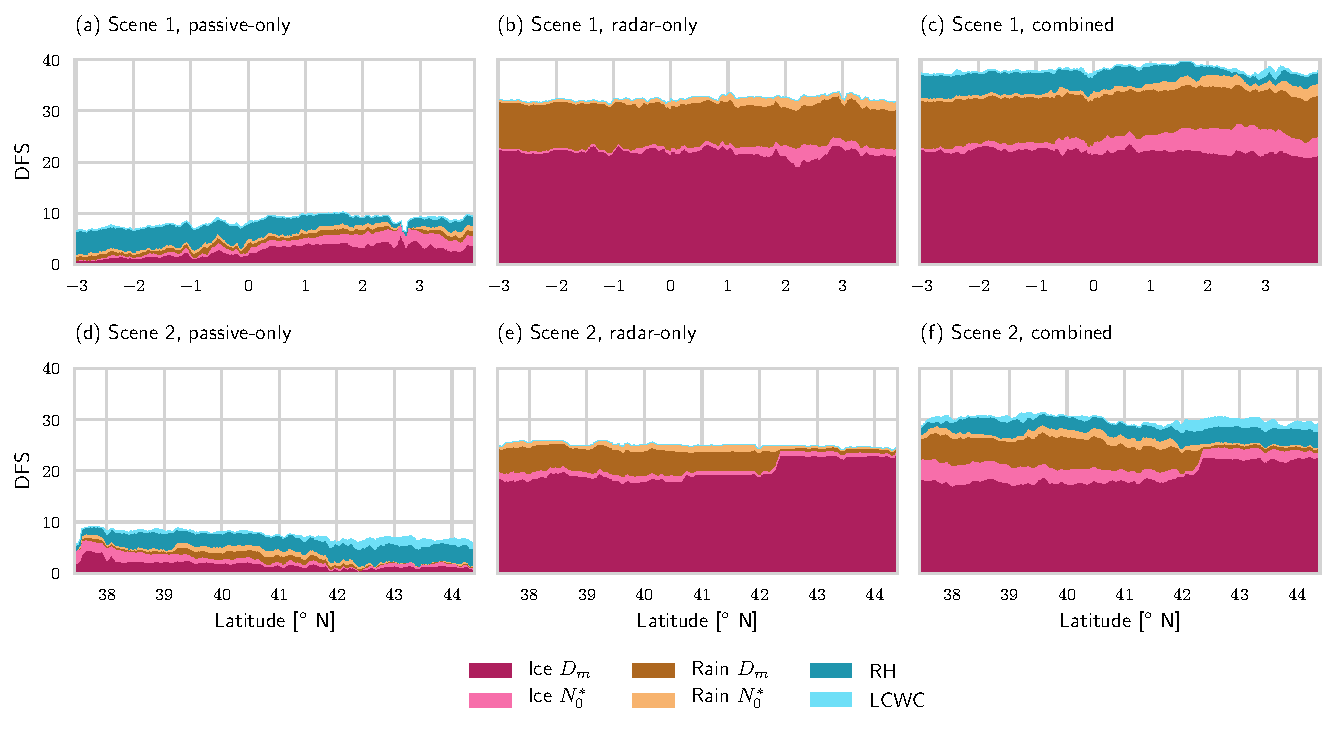
\includegraphics[width=\textwidth]{../plots/dfs}
\caption{Degrees of freedom for signal for all retrieval configurations and both
  test scenes obtained with the Large Plate Aggregate model. The colored areas
  in each plot represent the contribution to the cumulative degrees of freedom
  from each retrieval quantity. Results for the first and second test scene
  are displayed in the first and second row, respectively. The first, second
  and third panel in each row show the results for the passive-only, radar-only
  and the combined retrieval.}
\label{fig:dfs}
\end{figure}

\subsection*{Reviewer comment 4}

The manuscript is rather lengthy making it difficult for the reader to
extract the majorpoints. I strongly suggest a) to move part of the analysis into
an appendix (, b) remove double statement (see minor comments, also the LWC
plot) and c) to remove figurecaption like information (for example L92 or
“filled contours”) from the text. The text must make sense without looking at
the figure. Figure only support the statements made in the text. Lengthy
descriptions such as ``The plot shows..'' need to be avoided.

\subsubsection*{Author response}

We have followed  the referee's recommendations to make the manuscript more
concise.

\subsubsection*{Changes in manuscript}

\begin{itemize}
\item Descriptions of the figures which display the results in Sect.~3 have
  been removed.
\item The analysis of the results from the second test scene have been
  moved to an appendix.
\end{itemize}

\section{Minor comments}
\subsection*{Reviewer comment 1}

L39: Is sensitivity really the right word? Range resolution is the main
advantage –signal-to noise range depends on distance and hydrometeor
distribution,

\subsubsection*{Author response}

Following the reviewer's suggestion the sentence has been rewritten.

\subsubsection*{Changes in manuscript}

Most of the introduction has been rewritten and the corresponding
expression has been removed.

\subsection*{Reviewer comment 2}

L48: MWI will also cover new spectral channels, e.g. 118 GHz

\subsubsection*{Author response}

The $118\ \unit{GHz}$ spectral band is employed already today by the FY-3
satellites. Nevertheless, we mention the band now also in the introduction.

\subsubsection*{Changes in manuscript}

\begin{change}[63]
 MWI will complement ICI's observations with measurements at traditional
 millimeter wavelengths \DIFaddbegin \DIFadd{as well as a spectral band around
   the $118\ \unit{GHz}$ oxygen line}\DIFaddend . The observations of MWI, which
 cover the frequency range from $19\ \unit{GHz}$ up to $183\ \unit{GHz}$, will
 provide additional sensitivity to liquid and frozen precipitation as well as
 water vapor.
\end{change}

\subsection*{Reviewer comment 3}

L62: “high-resolution” is always relative for a model. I would recommend avoiding this term and use Cloud resolving Model (CRM).

\subsubsection*{Author response}

The proposed improvement has been adopted in the revised version of the manuscript.


\subsubsection{Changes in manuscript}

\begin{change}[75]
  \DIFaddbegin \DIFadd{For this, a combined, variational retrieval is
    developed and applied to simulated observations of }\DIFaddend scenes from a
  \DIFdelbegin \DIFdel{high-resolution atmospheric model and used to further
    explore the synergies between the active and passive observations.
  }\DIFdelend \DIFaddbegin \DIFadd{cloud-resolving model (CRM).}\DIFaddend
\end{change}


\subsection*{Reviewer comment 4}

L68:  After you mention GPM (with scanning radar) it might be good to say that you are only looking at a nadir pointing radar (curtain).  The swath center came bit as a surprise.

\subsubsection*{Author response}

The radar type is now stated more explicitly in the introduction.

\subsubsection*{Changes in manuscript}

\begin{change}[75]
\DIFaddbegin \DIFadd{An airborne viewing geometry is assumed for the simulations
  with all sensors pointing at nadir and close-to overlapping antenna
  beams.}\DIFaddend
\end{change}
%To incorporate the proposed improvement the corresponding sentence has been
%modified as follows:
%
%{\itshape This work applies the concept of synergistic radar and sub-millimeter radiometer
%retrievals to the upcoming ICI and MWI sensors by combining them with a
%conceptual, nadir-pointing W-band cloud radar.}

\subsection*{Reviewer comment 5}

L70: There has been quite some literature about combining active and passive
MW using a Bayesian framework which should be acknowledged, e.g. Grecu, M., \&
Olson,W. S. (2006), Johnson et al. (2012) , Munchak, S. J., \& Kummerow

\subsubsection*{Author response}

A paragraph listing previous work on synergistic retrievals using radar and
passive radiometers at lower microwave frequencies has been added to the
introduction.

\subsubsection*{Changes in manuscript}

\begin{change}[51]
\DIFadd{Prominent examples of satellite missions that exploit both of these
  synergies are the the Tropical Rainfall Measuring Mission (TRMM,
  \mbox{ \citet{kummerow98, grecu04, munchak11}}\hspace{0pt}
    ) and the Global Precipitation Measurement (GPM, \mbox{
      \cite{hou14, grecu16, kummerow15}}\hspace{0pt} ) mission. Since
    the principal target of these missions are retrievals of liquid
    hydrometeors, they make use of sensors at comparably low microwave
    frequencies and hence provide only limited sensitivity to frozen
    hydrometeors}\DIFaddend .
\end{change}


%Following the suggestion of the reviewer, the following paragraph will be added to the introduction:
%
%{\itshape
%\ldots has been
%investigated \citep{evans05, jiang19}.
%
%Combined retrievals using radar and passive radiometer observations, have also
%been developed for the Tropical Rainfall Measuring Mission (TRMM,
%\citet{kummerow98, grecu04}) and the Global Precipitation Measurement (GPM,
%\citet{hou14, grecu16, munchak11}) mission. However, since the principal target
%of these missions were liquid hydrometeors, they make use of sensors at
%comparably low microwave frequencies, which provide only limited sensitivity to
%frozen hydrometeors.
%
%This work \ldots
%}


\subsection*{Reviewer comment 6}

L84: Test scenes have a grid resolution of 1 km horizontally. As this is not the
true model resolution I would have recommended to coarse sample the model data
(maybe every 5th data point) and include more diverse profiles instead. This
might be especially interesting for the scatter plots.

\subsubsection*{Author response}

The point raised by the reviewer here is certainly correct. However, the
decision to restrict simulations to two test scenes was motivated primarily by
the computational costs of performing the retrievals. The scatter plot in
Fig.~10 (shown in Fig.~\ref{fig:results_scatter_b} in this document), which was
unfortunately missing from the manuscript , shows that the emergent structures
are consistent for both test scenes. This indicates that the scenes cover
sufficient profile variability to be statistically representative.

\subsection*{Reviewer comment 7}

Motivation lacking: “To perform RT simulations for each GEM profile the PSD
needs to be diagnosed from the prognostic GEM variables, i.e. N and m..”

\subsubsection*{Author response}

The corresponding paragraph has been rewritten and the sentence removed.

%To address another comment by another reviewer the paragraph containing the sentence
%will be rewritten and the sentence removed.
%
%{\itshape The prognostic parameters of the two-moment scheme are the slope and
%  intercept parameters of the distribution, which are derived from the mixing
%  ratios and number densities predicted by the GEM model. The third parameter of
%  the PSD and the mass-size relationship of each hydrometeor class are set to
%  fixed, class-specific values. The parameters of the mass-size relationships
%  are given in Tab.~\ref{tab:species_parameters}. The masses of all ice
%  particles in the model are assumed to scale with a power of three, which leads
%  to high densities for large particles.}


\subsection*{Reviewer comment 8}

L92:“prognoses”   means   forward   in   time   -   you   mean   diagnosed,   calculated,
determined.

\subsubsection*{Author response}

The corresponding paragraph has been rewritten and the sentence removed.

%{\itshape The four panels display the derived particle size distributions for the
%  four frozen hydrometeor types together with renderings of the particle shapes
%  used in the forward simulations.}


\subsection*{Reviewer comment 9}

L98: I find the term “horizontal and vertical scaling” strange – why not saying
PSD shape is similar but scaling in respect to diameter and number density. At
least definethe term clearly the first time that you use it or define a short
for it.

\subsubsection*{Author response}
 
C.f. Comments from Referee 1 - Reviewer comment 2.

\subsection*{Reviewer comment 10}

L103: model test – be careful also at other instances that “model” can mean too manythings. Here I would say GEM test scenes.

\subsubsection*{Author response}

Since much of the manuscript has been rewritten, this exact sentence is not
present anymore. However, attention has been paid to the use of the word model
and to ensure that its interpretation is unambiguous.

%by
%changing the sentence as follows:
%
%{\itshape
%The simulations apply the same microphysics scheme
%as the GEM test scenes, which means that they use the same six hydrometeor classes
%and PSD parametrizations.}


\subsection*{Reviewer comment 11}

L119: Need to clearly say that polarization effects are neglected though these can beseveral Kelvin, e.g.  Xie et al., 2015.  You ignore this effect but even consider noise reduction.


\subsubsection*{Author response}

C.f. Comments from Referee 2 - General comment 2.

%{\itshape In order to reduce the complexity of generating simulated observations, a number
%of simplifications are applied to the viewing geometry and the radiative
%transfer modeling. The beams of all three sensors are assumed to point at nadir
%and to be perfectly coincident pencil beams. In this way, observations for the
%GEM model scenes can be simulated by performing a single 1-dimensional radiative
%transfer calculation for each profile. Moreover, multiple scattering effects in
%the radar observations are neglected. The simulations therefore do not take into
%account beam filling effects caused by atmospheric inhomogeneity across the
%footprints of the different sensors. The incidence angles of the beams of ICI
%and MWI will be around $53^\circ$ at the Earth's surface, so the simulations
%performed here do not represent the viewing geometry of a space-borne
%configuration involving ICI and MWI accurately. Realistic modeling of the
%viewing geometry as well as multiple scattering effects in a variational
%retrieval are currently not feasible at reasonable computational cost with the
%tools used in this study. Assuming observations at nadir further allows neglecting
%polarization effects, which can be several Kelvin at typical viewing geometries
%of imager sensors \cite{xie15}. Since the focus of this study are the fundamental
%synergies between the active and passive observations, this was deemed
%sufficient for its scope. Moreover, these assumptions are justifiable for
%air-borne observations, which adds practical relevance to the simulations.}



\subsection*{Reviewer comment 12}
L157-159: needs to be better motived, references?

\subsubsection*{Author response}

To provide  better motivation for the use of the $\chi^2$ statistic
the text given below been added to the manuscript.

\subsubsection{Changes in manuscript}

\begin{change}[158]
\DIFdel{To assess the }\DIFdelend \DIFaddbegin \DIFadd{The }\DIFaddend quality
of a retrieved state $\hat{\mathbf{x}}$ and corresponding simulated \DIFdelbegin
\DIFdel{observation }\DIFdelend \DIFaddbegin \DIFadd{observations }\DIFaddend
$\hat{\mathbf{y}} = \mathbf{F}(\hat{\mathbf{x}})$ \DIFdelbegin \DIFdel{, we
  define }\DIFdelend \DIFaddbegin \DIFadd{is assessed using }\DIFaddend the
following diagnostic quantity\DIFaddbegin \DIFadd{:}
\DIFaddend
\begin{align} \chi^2_y &= \DIFdelbegin \DIFdel{\delta }\DIFdelend
  \DIFaddbegin \DIFadd{\Delta }\DIFaddend \mathbf{y}^T \mathbf{S}_e^{-1}
  \DIFdelbegin \DIFdel{\delta }\DIFdelend \DIFaddbegin \DIFadd{\Delta
  }\DIFaddend \mathbf{y} \DIFdelbegin \DIFdel{, }\DIFdelend
\end{align}
\DIFdelbegin \DIFdel{where $\delta \mathbf{y} = \mathbf{y} -
  \hat{\mathbf{y}}$}\DIFdelend  \DIFaddbegin \DIFadd{Here, $\Delta
\mathbf{y} = \mathbf{y} - \hat{\mathbf{y}}$ is the difference between the fitted
and true observations and $\mathbf{S}_e$ is the covariance matrix describing the
measurement errors}\DIFaddend . The quantity $\chi^2_y$ \DIFdelbegin \DIFdel{is
  here used to approximate a $\chi^2$-test for the misfit between the
  observations $\mathbf{y}$ and the retrieval fit $\hat{\mathbf{y}}$. Although a
  formally correct }\DIFdelend \DIFaddbegin \DIFadd{corresponds to the sum of
  squared errors in the fitted observations weighted by the uncertainties in
  each channel or range bin. It should be noted that the quantity has no
  meaningful interpretation in terms of }\DIFaddend $\chi^2$\DIFdelbegin
\DIFdel{-test for $\delta\mathbf{y}$ should apply a different covariance matrix
}\DIFdelend \DIFaddbegin \DIFadd{-statistic for the errors in the fitted
  observations since they will neither be independent }\DIFaddend (c.f.
Chapter~12 in \cite{rodgers00}) \DIFdelbegin \DIFdel{, such tests were found
to yield very high values that deviate strongly from the expected chi-square
distribution. The $\chi^2_y$ value used here provides a less strict test in the
sense that it will generally be smaller than if the formally correct covariance
matrix was used.
}%DIFDELCMD < 

%DIFDELCMD < %%%
\DIFdel{The amount of information contained in a retrieval can be quantified by
computing the degrees of freedom for signal (DFS). Let $\mathbf{K} \in
\mathbb{R}^{m \times n}$ be the Jacobian of the forward model $\mathbf{F}$. Then
the DFS of the observations can be computed as the trace of the averaging kernel
matrix
}\begin{eqnarray*}
  \DIFdel{\mathbf{A} }&\DIFdel{=(\mathbf{K}^T\mathbf{S}_e^{-1}\mathbf{K} + \mathbf{S}_a^{-1})^{-1}
  \mathbf{K}^T\mathbf{S}_e^{-1}\mathbf{K}.
}\end{eqnarray*}
\DIFdelend \DIFaddbegin \DIFadd{nor Gaussian due to the presence of forward
model error. The value is therefore used here solely as a heuristic to quantify
the goodness of the fit to the true observations.
}\DIFaddend 

\end{change}


%The $\chi^2$ value defined in the manuscript corresponds to the component of the OEM cost that
%is related to the misfit in the observation vector. We use this value here as a heuristic
%to asses the goodness of the retrieval fit. Since neither the a priori distribution nor the
%observation error can be assumed to be Gaussian, applying a true $\chi^2$-test is not really
%meaningful. Similar applications can for example be found in \citet{duncan16}.

%To state this more clearly in the manuscript, the following changes will be introduced:
%
%{\itshape The quantity $\chi^2_y$ corresponds to the squared error in the fitted
%  observations weighted by the uncertainties in each channel. It should be noted
%  that the quantity has no meaningful interpretation in terms of
%  $\chi^2$-statistic for the errors in the fitted observations since they will
%  neither be independent (c.f. Chapter~12 in \cite{rodgers00}) nor Gaussian due
%  to the presence of forward model error. The value is used here as a heuristic
%  to quantify the goodness of the fit to the true observations.}


\subsection*{Reviewer comment 13}
L172: I doubt that the model has constant vertical resolution.  It will be better close to the surface and worse aloft. This should be mentioned than GEM is introduced.

\subsubsection*{Author response}

As suggested by the reviewer, this is mentioned in the revised manuscript when
the GEM test scenes are introduced. Moreover, a sketch will be added to the
manuscript which displays the GEM model grid and the grids of all retrieval
quantities for the retrievals.

\subsubsection*{Changes in manuscript}

The following text has been added to the description of the model scenes.

\begin{change}[92]
\DIFadd{ The vertical resolution of the model scenes varies between 250 and
  $500\ \unit{m}$ below an altitude of $18\ \unit{km}$ and decreases steadily
  above that.}\DIFaddend
\end{change}

In addition to this, the figure shown in Fig.~\ref{fig:retrieval_sketch} has been added
in Sect.~2.3.2 of the revised manuscript.

%This is indeed the case. To make this clear to the reader the following sentence
%is introduced in the paragraph describing the GEM model scenes:

%{\itshape The vertical resolution of the model scenes varies between 250
%and $500\ \unit{m}$ below an altitude of $18\ \unit{km}$ and decreases
%steadily above that.}
%
%Furthermore, to address the Reviewer comment 13 a figure will be added to
%the manuscript, which displays the model grid and the grids at which
%the different retrieval quantities are retrieved.

\subsection*{Reviewer comment 14}

L 174: for all hydrometeor species of the model? It would be helpful to first
introduce all retrieval quantities – I was missing a motivation for the
paragraph around L195. How do you define the freezing level (and later the
troposphere)? How do they vary in both test scenes? The model also likely has
supercooled liquid water above the freezing layer – how is this treated?

\subsubsection*{Author response}

For the simulated observations, supercooled liquid is treated in just the same
way as liquid water below the freezing level. As described in the paragraph
around L. 211, cloud liquid water in the retrieval is treated as purely
absorbing and simulated using a parametrized absorption model. Moreover, it is
restricted to temperatures of $230\ \unit{K}$ and up.

\subsubsection*{Changes in manuscript}

Fig.~\ref{fig:retrieval_sketch} has been added to the manuscript, which
displays all retrieval variables as well as the freezing level and the tropopause.
Moreover, the following text explaining the definitions of freezing level and
tropopause has been added to the manuscript:

\begin{change}[193]
As additional constraints, the retrieval of frozen hydrometeors is
restricted to the region between the freezing \DIFdelbegin \DIFdel{layer and the tropopause, whereas the
retrieval of liquid }\DIFdelend \DIFaddbegin \DIFadd{level, here defined simply as the
$273.15\ \unit{K}$-isotherm, and the approximate altitude of the tropopause. The
altitude of the tropopause is approximated as the first grid point at which the
lapse rate is negative and temperature below $220\ \unit{K}$. The retrieval of
rain }\DIFaddend hydrometeors is restricted to below the freezing \DIFdelbegin \DIFdel{layer. }%DIFDELCMD < 

%DIFDELCMD < %%%
\DIFdel{To further regularize the retrieval , $N_0^*$ for ice is retrieved at only 10
equally-spaced grid points between freezing layer and the tropopause. Similarly,
$D_m$ and }\DIFdelend \DIFaddbegin \DIFadd{level.}\DIFaddend
\end{change}

%In order to provide a better overview over the retrieval variables and
%grid resolutions the following sketch of the different retrieval setups has
%will be included in the revised version of the manuscript:
%
%\begin{figure}
%\centering
%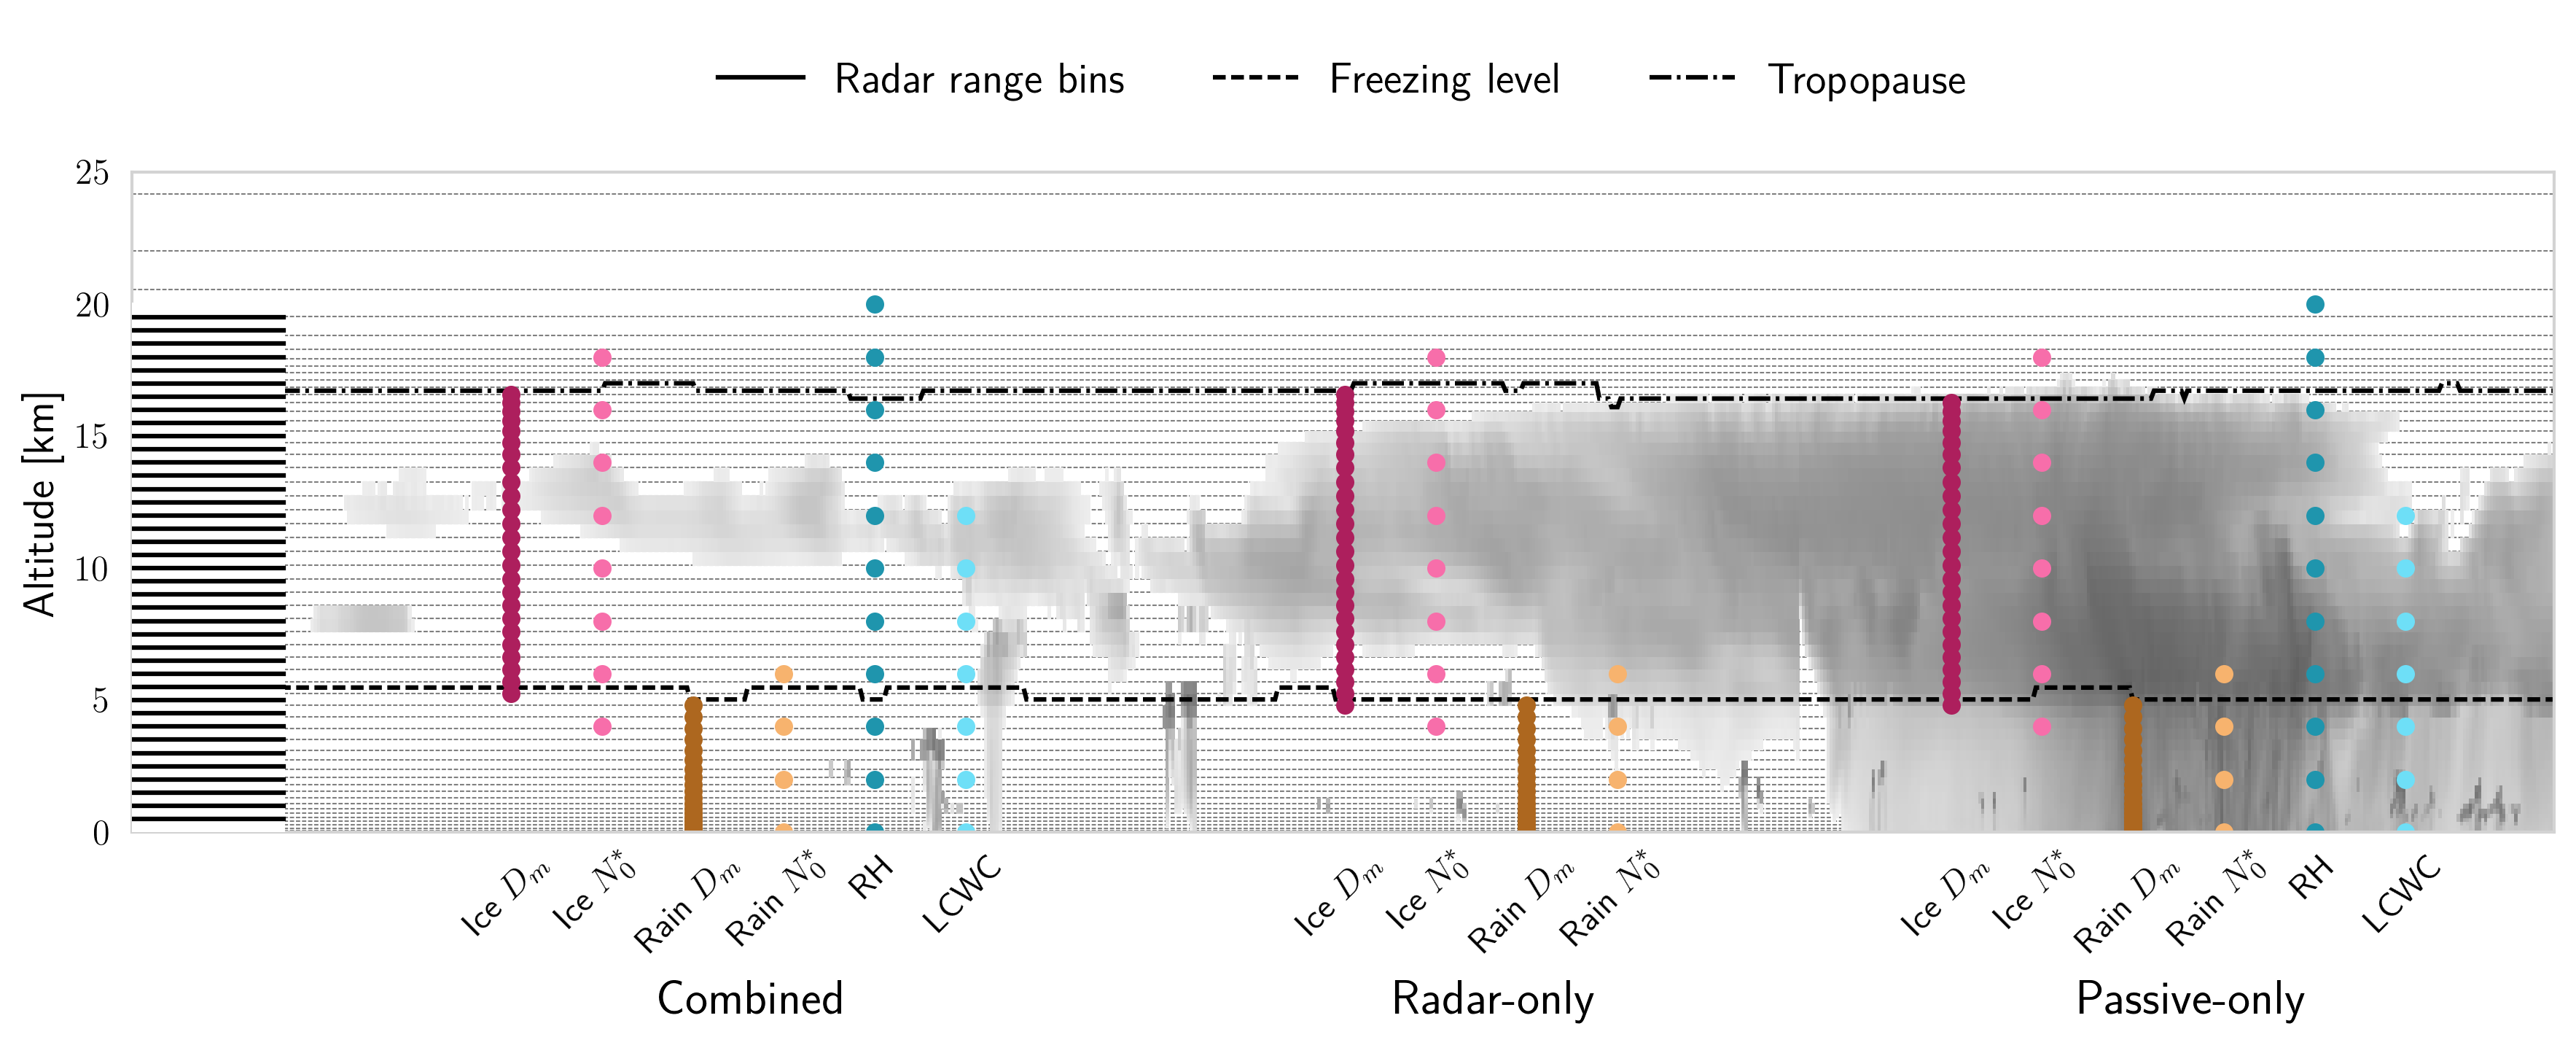
\includegraphics[width = 0.8\linewidth]{../plots/retrieval_sketch}
%\caption{Illustration of the retrieval quantities and their respective retrieval
%  grids. Grey, dashed lines show the resolution of the GEM model data while the
%  filled circles represent the grid points of the different retrieval
%  quantities. Panel (a) shows the configuration used in the radar-only and
%  combined retrieval. Panel (b) shows the configuration used in the passive-only
%  retrieval}
%\label{fig:retrieval_sketch}
%\end{figure}
%
%The motivation for retrieving $N_0^*$ in log-space is that its a priori
%distribution is more similar to a Log-normal rather than a Gaussian distribution
%(see for example \citet{delanoe14}). Since typical values for $D_m$ follow a
%Gaussian distribution rather well these values are retrieved in linear space.
%
%The handling of supercooled liquid in the GEM model scenes is similar to that
%of all other hydrometeors and therefore not explicitly mentioned. In the retrieval,
%liquid cloud is allowed to exist between the surface and the $240\ unit{K}$ isotherm
%and thus also represents supercooled clouds.


\subsection*{Reviewer comment 15}

L 198: Vertical resolution of retrieval grid: Why 4 points? The freezing layer
must be very different for both cased. Maybe a sketch would be helpful as later
on lines 230 the different vertical resolutions for other variables is discussed?

\subsubsection*{Author response}

We have revised the retrieval implementation and now use fixed retrieval grids
with a resolution of  $2\ \unit{km}$ for the $N_0^*$ parameters. Reducing the
resolution of the retrieval grids for the $N_0^*$ parameters was found to aid
the convergence of the retrieval.

\subsubsection*{Changes in manuscript}

The sketch requested by the reviewer has been added to the manuscript (c.f.
comment above).

\subsection{Reviewer comment 16}

L281: How do I know that Large Plate is the best performing model? Which parameter,plot, table does show that?

\subsubsection*{Author response}

This sentence has been removed from the revised version of the manuscript.

\subsection*{Reviewer comment 17}
L283-L307: Can be shortened significantly

\subsubsection*{Author response}

The proposed change has been adopted in the revised version of the manuscript.

\subsubsection*{Changes in manuscript}

\begin{change}[304]
\DIFadd{The $\chi^2_y$ values of the three retrieval configurations, displayed in }\DIFaddend Panel
(a)\DIFdelbegin \DIFdel{of the figure displays the $\chi^2_y$ value (normalized by the
dimension of the measurement space) for each profile in the scene. A high value
of $\chi^2_y$ indicates that the retrieved state is not consistent with the
input observations. The $\chi^2_y$ value for }\DIFdelend \DIFaddbegin \DIFadd{, give an indication of how well the retrievals are able to fit the
observations. For }\DIFaddend the radar-only retrieval\DIFdelbegin \DIFdel{is
remarkably low throughout most }\DIFdelend \DIFaddbegin \DIFadd{, the values are much smaller than 1
for most parts }\DIFaddend of the scene\DIFdelbegin \DIFdel{. This may indicate that the
retrieval is insufficiently regularized, allowing it to fit the noise in the observations. The }\DIFdelend \DIFaddbegin \DIFadd{, while for the }\DIFaddend passive-only and combined retrieval
\DIFdelbegin \DIFdel{, on the contrary, have a
normalized $\chi^2_y$ value around 1 over most of the scene. Since the presented
values are normalized, the value 1 corresponds to }\DIFdelend \DIFaddbegin \DIFadd{they are around }\DIFaddend the expected value of \DIFdelbegin \DIFdel{the
approximated chi-square distribution of $\chi^2_y$. All three retrievals exhibit
a region of elevated $\chi^2_y$ values near the core of the convective system.
In particular the high values of }\DIFdelend \DIFaddbegin \DIFadd{1. This indicates that the radar-only
retrieval overfits the observations, while }\DIFaddend the passive-only and combined
retrievals \DIFdelbegin \DIFdel{indicate that the retrieval was not able to find a good fitto the observations
here.
}%DIFDELCMD < 

%DIFDELCMD < %%%
\DIFdel{Panel (b) displays the retrieved column-integrated IWC, the ice water path
(IWP). The IWP is given in $\unit{dB}$ relative to the reference IWP since, owing to the high dynamic range of the reference values, }\DIFdelend \DIFaddbegin \DIFadd{achieve the expected fit. The exception is }\DIFaddend the \DIFdelbegin \DIFdel{curves could
otherwise not be distinguished.
Although all methods reproduce the reference
IWP fairly well, the combined retrieval yields the best overall agreement with
}\DIFdelend \DIFaddbegin \DIFadd{region around
$3^\circ\ N$, where the cloud is particularly thick and consists of a mix of
different hydrometeor types. Here, especially the passive-only retrieval has
problems fitting the observations.
}

\DIFadd{In terms of IWP, all methods provide fairly good estimates of }\DIFaddend the reference
values \DIFdelbegin \DIFdel{. Exceptions are the regions of high $\chi^2_y$ values where
the }\DIFdelend \DIFaddbegin \DIFadd{with the combined retrieval consistently yielding the smallest deviations.
Larger differences between the methods are observed when comparing the }\DIFaddend retrieval
\DIFdelbegin \DIFdel{failed to find a good fit to the observations.
}%DIFDELCMD < 

%DIFDELCMD < %%%
\DIFdel{Panel (c) shows the IWC field retrieved using the passive-only retrieval
.
Despite a certain resemblance in the overall structure between the retrieved and
reference IWCfield, the results do not reproduce }\DIFdelend \DIFaddbegin \DIFadd{results in terms of IWC. While }\DIFaddend the vertical structure of the cloud \DIFdelbegin \DIFdel{very well. It should be noted, however, that the displayed mass-density
range extends below the sensitivity limit of the passive-only observations
around $10^{-5}\ \unit{kg\ m^{-3}}$ (c.f. Fig.~4), which explains
the smeared-out appearance of the
results to some extent.
}%DIFDELCMD < 

%DIFDELCMD < %%%
\DIFdel{The }\DIFdelend \DIFaddbegin \DIFadd{is captured
only very roughly by the passive retrieval, it is better resolved by the
}\DIFaddend radar-only \DIFdelbegin \DIFdel{results, shown in panel (d), reproduce the vertical structure of
the cloud well. Nonetheless, when compared to the reference IWC field, certain
discrepancies are visible: The }\DIFdelend \DIFaddbegin \DIFadd{and the combined retrieval. On closer inspection, however, it becomes
evident that the }\DIFaddend radar-only retrieval \DIFdelbegin \DIFdel{tends to overestimate the
mass density at the bottom }\DIFdelend \DIFaddbegin \DIFadd{deviates systematically from the reference
IWC in specific regions }\DIFaddend of the cloud\DIFdelbegin \DIFdel{and underestimate the mass
concentrations at the top }\DIFdelend \DIFaddbegin \DIFadd{, such as for example the upper part }\DIFaddend of the
cloud \DIFdelbegin \DIFdel{.
}%DIFDELCMD < 

%DIFDELCMD < %%%
\DIFdel{The results of the combined retrieval are displayed in panel (e). Although some
artifacts are clearly visible in the
retrieved IWC field, the retrieval
reproduces the vertical structure well. In particular, }\DIFdelend \DIFaddbegin \DIFadd{between $0^\circ N$ and $2^\circ N$. These deviations are corrected in the
results from }\DIFaddend the combined retrieval\DIFdelbegin \DIFdel{succeeds to correct some of the systematic deviations of the radar-only
retrieval : The mass density at cloud base is reduced and increased at cloud top}\DIFdelend \DIFaddbegin \DIFadd{, although certain retrieval artifacts are
visible}\DIFaddend .
\end{change}

%Following the reviewers recommendations the section will be shortened and
%now  reads as follows:
%
%{\itshape
%Results of the retrieved water content for the first test scene are displayed in
%Fig.~\ref{fig:results_a}. The corresponding results from the second test scene
%are included in Appendix~\ref{app:results_b}. The reference water content is
%defined here as the sum of the masses of the four frozen hydrometeor species in
%the GEM model scenes.
%
%The $\chi^2_y$ value of the different methods, displayed
%in Panel (a), gives an indication of how well the retrievals were able to fit
%the observations. For the radar-only retrieval, the values are far below 1
%for most parts of the scene, while for the passive-only and combined retrieval
%the around 1. This indicates that all methods fitted the observations well over
%the whole scene except for the region around $3^\circ\ N$, where the cloud
%is particularly thick.
%
%In terms of IWP, all methods provide fairly good estimates of the reference IWP
%with the combined retrieval consistently yielding the smallest deviations.
%Larger differences between the methods are observed when comparing the retrieval
%results in terms is IWC. While the vertical structure of the cloud is captured
%only very roughly by the passive retrieval, it much better resolved by the
%radar-only and the combined retrieval. On closer inspection, however, it becomes
%evident that the radar-only retrieval deviates systematically from the reference
%IWC in specific regions of the cloud, such as for example the upper part of the
%cloud between $0^\circ N$ and $2^\circ N$. These deviations are corrected in
%the results from the combined retrieval, although certain retrieval artifacts
%are visible here.}


\subsection*{Reviewer comment 18}
L332: There can I see that? Give figure?

\subsubsection*{Author response}

The sentence has been removed from the revised version of the manuscript.

\subsection*{Reviewer comment 19}
L325: The two paragraph here give similar information -> streamline

\subsubsection*{Author response}

The proposed change have be adopted in the revised version of the manuscript.

\subsubsection*{Changes in manuscript}

\begin{change}[508]
\DIFdel{Similar to the radar-only retrieval, the results of the combined retrieval are
located close to the diagonal.
But the clusters observed in the radar-only
results are to large extent merged in the combined results. Moreover, except for the results obtained with the GemCloudIce particle shape, the two clusters move
in closer towards the diagonal. The combined retrieval thus improves the IWC
retrieval for the specific hydrometeor species in the scene.
}\DIFdelend \DIFaddbegin \DIFadd{is biased for specific hydrometeor classes. In the combined
and even the passive-only results, this effect is weaker and the clusters are
generally moved towards the diagonal. For graupel, all retrievals perform badly
but this is likely due to it being present only in the core of the convective
system where the signals from all sensors can be expected to be saturated.
}\DIFaddend 

\DIFdelbegin \DIFdel{Nonetheless, the results for the GemCloudIce particle stand out in the }\DIFdelend \DIFaddbegin \DIFadd{Comparing the }\DIFaddend results \DIFdelbegin \DIFdel{.
Even though the systematic deviations observed in }\DIFdelend \DIFaddbegin \DIFadd{for different particle models, a clear dependency is
evident in the passive-only and the combined results while }\DIFaddend the radar-only
retrieval \DIFdelbegin \DIFdel{are
reduced for most particle shapes, for this specific shape they are instead
increased. The retrieval error is particularly large for snow, which is strongly
underestimated for reference mass concentrations around $10^{-4} \ \unit{kg\ m^{-3}}$.
}%DIFDELCMD < 
\end{change}

%To make the description of the results from the scatter plots more
%concise the section will rewritten as follows:
%
%{\itshape
%Not surprisingly, the results from the
%passive-only retrieval exhibit the strongest deviations from the diagonal. Since
%the passive channels alone contain only limited information on the vertical
%distribution of ice in the atmosphere, the retrieval cannot be expected to yield
%accurate results at the resolution considered here. Although rather weak, a
%certain effect of the ice particle model on the retrieval results can be
%observed. In particular, the GemCloudIce model leads to a systematic
%underestimation of ice mass densities, which are less pronounced for the other
%particle models.
%
%In terms of overall accuracy, i.e. systematic deviations from the diagonal, no
%clear differences between the three configurations are visible. The color-coding
%reveals, however, that the radar-only retrieval is biased for specific
%hydrometeor classes. This effect is less pronounced for the combined retrieval
%and seem to be weaker also in the passive-only results. For Graupel, both the
%radar-only and the combined retrieval perform badly but this due to the radar
%signal saturating in the regions of the scene where Graupel is present (c.f.
%Fig.~\ref{fig:overview} and Fig.~\ref{fig:observations_a}).
%
%Results of all retrievals are affected by the choice of the ice particle model,
%which can cause systematic deviations especially at high IWC values. For the
%radar-only results these deviations are smallest for the LargeColumnAggregate,
%whereas for the combined retrieval the LargePlateAggregate and 8-ColumnAggregate
%yield the most accurate results.}


\subsection*{Reviewer comment 20}
L333-344: I would put this to the appendix

\subsubsection*{Author response}

Following the reviewer's advice, the analysis of the second test scene
has been moved to the appendix.


\subsection*{Reviewer comment 21}
L444: Here it needs to be made clearer how this goes beyond what GPM is doing.

\subsubsection*{Author response}

To clarify how our work goes beyond what GPM a paragraph detailing this
has been added to the discussion.

\subsubsection*{Changes in manuscript}
\begin{change}[421]
\DIFaddbegin \DIFadd{The novelty of this work for lies, in part, in the application of ICI's
sub-millimeter channels, which sets it apart from the combined retrievals
developed for the TRMM and GPM missions. Moreover, the development of a fully
consistent variational retrieval in which all retrieval quantities are retrieved
simultaneously using observations from all sensors development is also novel.
This allows comparison of the synergistic retrieval to equivalent radar-only and
passive-only configurations and therefore a direct analysis of the synergies
between the active and passive observations.
}
\end{change}

%To clarify how our work goes beyond what GPM is doing the following paragraph
%will be added to the manuscript:
%
%{\itshape The novelty of this work lies, for one part, in the application of ICI's
%sub-millimeter channels, which sets it apart from the combined retrievals
%developed for the TRMM and GPM missions. For the other part, it lies in the
%development of a fully-consistent variational retrieval in which all retrieval
%quantities are retrieved from the observations from all sensors simultaneously.
%This allows comparing the retrieval to equivalent radar-only and passive-only
%configurations and therefore a direct analysis of the synergies between the
%active and passive observations.}

\subsection*{Reviewer comment 22}
L495:  “does not say much about the general validity of the assumption”.   Here you should dig in a bit more. What is the role of a priori and covariances?

\subsubsection*{Author response}

Following the suggestion of the reviewer we will  the discussion
of the a priori assumptions has been extended.

\subsubsection*{Changes in manuscript}

C.f. the first change listed for Comments from Referee 1 - General comment 1.

%To extend the discussion of the role of the a priori assumptions in the retrieval
%the corresponding paragraph will be modified as follows:
%
%{\itshape 
%  The a priori assumptions which were used in this study were similar but not
%  identical to what is used in the DARDAR retrievals. Also here it should be
%  noted, that the presented results should not be taken to be representative for
%  the DARDAR product. Rather than this, the DARDAR a priori settings were chosen
%  since they represent well established and validated assumptions for ice cloud
%  retrievals and therefore should provide a reasonable starting point for the
%  development of a combined cloud retrieval. Although the a priori assumptions
%  work well for the first test scene they lead to systematic error in the second
%  scene. The analysis in Fig.~\ref{fig:results_scatter} shows that the cause for
%  this is the composition of the cloud. The a priori works well if the scene
%  contains both snow and ice but causes systematic errors when this is not the
%  case. The role of the a priori is to complement the observations with additional
%  information in order to make the retrieval problem tractable. For the radar-only
%  retrieval this means that the a priori determines how the information from a
%  single range gate is distributed between the two degrees of freedom of the
%  particle size distribution. Since the degrees of freedom vary more or less
%  independently from each other, no a priori can fit for every possible cloud
%  configuration.
%}

\subsection*{Reviewer comment 23}
L560:  Rethink the bullet structure.  2.  Is not an independent result.  For each result refer to the part of the manuscript where you can clearly see that.  Especially result 3 should be detailed – how do ICI channel advance the currently available data?

\subsubsection*{Author response}

The bullet points have been removed in the revised manuscript and replaced
by a text which presents the conclusion in a logically coherent way.

\subsubsection*{Changes in manuscript}

\begin{change}[540]
The main \DIFdelbegin \DIFdel{conclusions from the results presented above are:
}%DIFDELCMD < \begin{enumerate}
%DIFDELCMD < \item %%%
\DIFdel{The complementary information in active and
passive microwave observations canconstrain two degrees of freedom of the
PSD }\DIFdelend \DIFaddbegin \DIFadd{conclusion from this work is that the combination of radar and
sub-millimeter radiometer observations can, to some extent, constrain both the
size and number concentration }\DIFaddend of frozen hydrometeors \DIFdelbegin \DIFdel{.
}%DIFDELCMD < \item %%%
\DIFdel{This reduces systematic retrieval errors for specific hydrometeor species whose
  properties are not well described by the a priori assumptions.
}%DIFDELCMD < \item %%%
\DIFdel{Especially the sub-millimeter channels of the ICI radiometer contribute to the synergistic information content for ice particles.
}%DIFDELCMD < \end{enumerate}
%DIFDELCMD < 

%DIFDELCMD < %%%
\DIFdel{In addition to this}\DIFdelend \DIFaddbegin \DIFadd{(Fig.~5).
The increased sensitivity of the combined retrieval to the microphysical
properties of hydrometeors helps to improve the accuracy of IWC retrievals and
avoid systematic errors observed in an equivalent radar-only retrieval
(Fig.~8, 9). Moreover}\DIFaddend , the combined
retrieval \DIFdelbegin \DIFdel{also shows improved profiling capabilities
for warm and supercooled liquid clouds}\DIFdelend \DIFaddbegin \DIFadd{showed clear sensitivity to particle number concentrations and was
able reproduce their vertical structure in regions where the cloud composition
is homogeneous (Fig.~10, 11)}\DIFaddend .

The results \DIFdelbegin \DIFdel{presented in this study }\DIFdelend particularly highlight the \DIFdelbegin \DIFdel{complementarity
of the active and passive observations
: Although the radar provides observations at high vertical resolution, they contain insufficient information on the
microphysical properties of hydrometeors . The passive-only observations, on the contrary, have low vertical resolution, but are more sensitive to cloud
microphysics allowing a
potentially more accurate IWP retrieval than what can be
obtained from the radar alone. A synergistic retrieval using both types of observations allows combining the high vertical resolution of the radar with the sensitivity to cloud microphysics }\DIFdelend \DIFaddbegin \DIFadd{importance of sub-millimeter observations
for combined retrievals of frozen hydrometeors. While observations at currently
available microwave frequencies provide information complementary to that from a
radar-only for thick clouds with very large particles ($D_m > 800\ \unit{\mu m},
\text{IWC} > 10^{-4}\ \unit{kg\ m^{-3}}$), frequencies above $200\ \unit{GHz}$
provide additional information on cloud microphysics (Fig.~\ref{fig:contours})
at smaller particles sizes and water content ($D_m > 200\ \unit{\mu m},
\text{IWC} > 10^{-5}\ \unit{kg\ m^{-3}}$).}
\end{change}


%To improve the presentation of the conclusions, the bullet points will be removed
%and the first paragraphs of the conclusions will be rewritten as follows:
%
%{\itshape The main conclusion from this work is that the combination of radar and
%  sub-millimeter radiometer observations allows to constrain both the size
%  as well as the concentration of frozen hydrometeors. The sensitivity of
%  the combined observations to the microphysics of the cloud reduced the
%  median bias in the retrieved IWC from more than $50\ \%$ in the radar-only
%  to less than $10\ \%$ for suitable choices of the particle model (Fig.~\ref{fig:boxes}).
%
%  Our results particularly highlight the importance of sub-millimeter observations
%  for combined retrievals of frozen hydrometeors. While observations at currently
%  available microwave frequencies provide only limited complementary information
%  to the radar observations, it is mainly the frequencies above $200\ \unit{GHz}$
%  that provide additional information on cloud microphysics (Fig.~\ref{contours})
%  for
%
%  Moreover it has been found that the combination of radar and passive microwave
%  observations may help the retrieval of mixed-phase clouds. Since the role of
%  these clouds in the climate of the arctic are an active topic of study, the use
%  of combined sub-mm/radar observations should be further investigated.}


\subsection*{Reviewer comment 24}

Fig.  3: Is it really worth having the slightly different size distribution shapes for frozen and liquid? Isn’t there a stronger difference between different frozen hydrometeors

\subsubsection*{Author response}

This is certainly true but in most clouds ice and rain can be distinguished
fairly well a priori, which simplifies treating them as different species using
different PSD shapes. Distinguishing between different frozen hydrometeors is
difficult to do a priori and using multiple species of hydrometeors in the
retrieval was found to cause ambiguities which the retrieval is not able to
resolve.


%We agree with the reviewer that the slightly different size distributions shapes likely do
%not affect the retrieval significantly. The choice of the PSD parameters for liquid
%hydrometeors was made rather arbitrarily, but since the retrieval was found to work
%the effect of the PSD parameters has not been investigated further.

\subsection*{Reviewer comment 25}
Figures 7 and 8:  I’m not sure why these are separate figures – it seems like allpanels could fit on one page.

\subsubsection*{Author response}

Figures 7 and 8 will be combined into a single figure in the revised manuscript.

\subsubsection*{Changes in manuscript}

C.f. Comments from Referee 1 - Specific comment 9.

\subsection*{Reviewer comment 26}
Fig. 4 and also in text: “cloud signal” say that this is dTB.

\subsubsection*{Author response}

Following the reviewers recommendation, the passive cloud signal will be
referred to in the text as $\Delta T_B$ and the radar signal as
$\text{dBZ}_\text{max}$.

\subsubsection*{Changes in manuscript}

Fig.~5 and its caption have been changed as shown
in Fig.~\ref{fig:contours}. In addition to this, the paragraph describing
the results has been changed as follows.

\begin{change}[272]

\DIFdelbegin \DIFdel{Figure~4 displays the simulated passive cloud signal , i.e. the
brightness
temperature difference between clear sky and cloudy sky simulation, as filled
contours for a selection of channels of the MWI and ICI sensors. For given
values of $N_0^*$ and $D_m$, the corresponding ice mass density is given by
the relation
}\begin{eqnarray*}
\DIFdel{m = \frac{\pi \rho}{4 ^ 4}N_0^* D_m^4.
}\end{eqnarray*}
%DIFAUXCMD
\DIFdel{In the figure, the cloud signal is displayed in $D_m$-mass density space and
thus shows how the measured passive cloud signal varies with the horizontal and
vertical scaling parameters of
the PSD.
Overlaid onto }\DIFdelend \DIFaddbegin \DIFadd{The cloud signal in the radiometer observations is the
difference between the cloudy- and clear-sky brightness temperatures ($\Delta
T_B$). The signal in the active observations is here defined as the maximum of
the measured profile of radar reflectivity $\text{dBZ}_\text{max}$.
Figure~4 displays }\DIFaddend the contours of \DIFdelbegin \DIFdel{the
passive cloudsignal are the isolines of the maximum radar reflectivity returned
from the cloud}\DIFdelend \DIFaddbegin \DIFadd{$\Delta T_B$ and
$\text{dBZ}_\text{max}$ with respect to $D_m$ and the cloud's water content,
which is proportional to $N_0^*$:
}\begin{align}
\DIFadd{\text{WC} = \frac{\pi \rho}{4 ^ 4}N_0^* D_m^4,
}\end{align}
\DIFadd{with $\rho$ the density of ice}\DIFaddend .
\end{change}


\begin{figure}
\centering
\DIFdelbeginFL %DIFDELCMD < \includegraphics[width = 0.8\textwidth]{figures/fig04}
%DIFDELCMD < %%%
\DIFdelendFL \DIFaddbeginFL 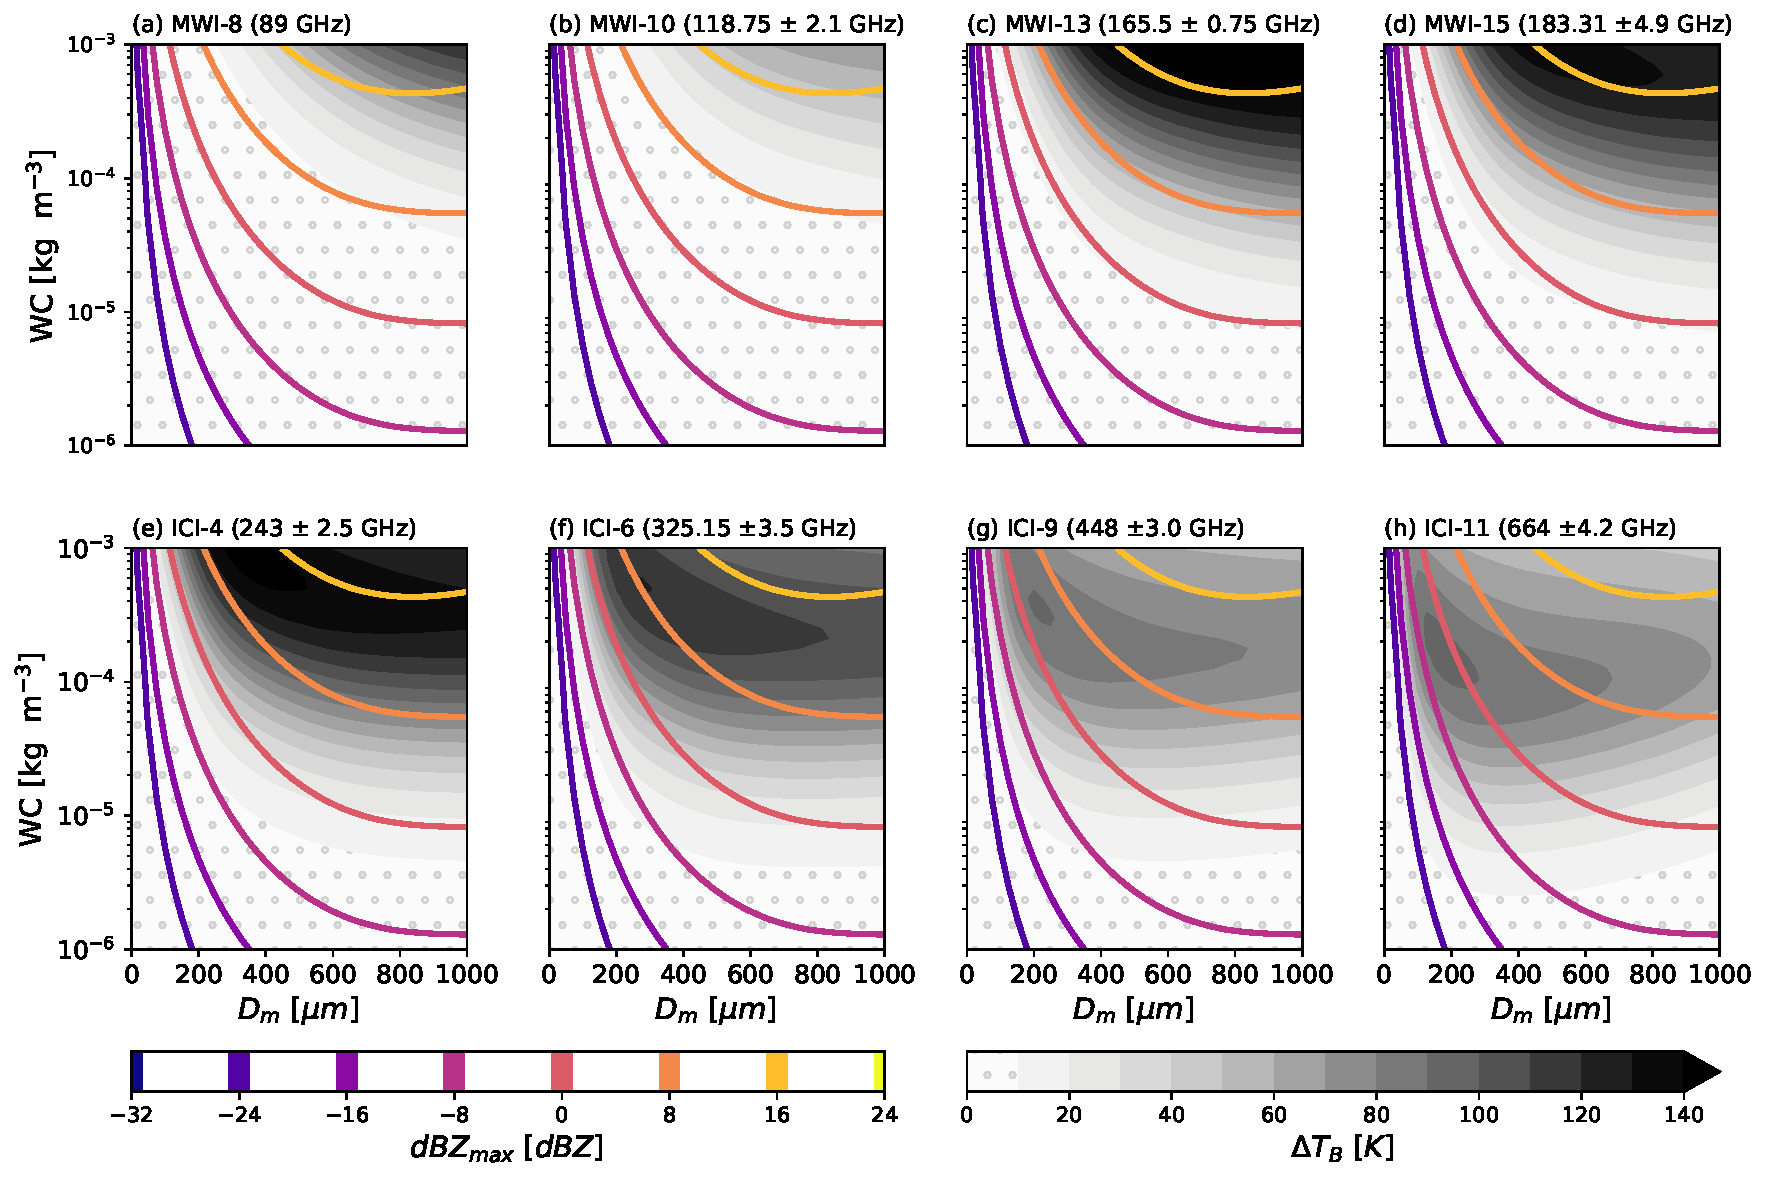
\includegraphics[width = 1.0\textwidth]{../plots/contours}
\DIFaddendFL \caption{Simulated observations of a homogeneous, $5\ \unit{km}$ thick cloud
  layer with varying water content $m$ and mass-weighted mean diameter $D_m$.
  The panels display the maximum radar reflectivity in dBZ
  \DIFaddbeginFL \DIFaddFL{($\text{dBZ}_\text{max}$) }\DIFaddendFL overlaid onto the cloud signal \DIFaddbeginFL \DIFaddFL{($\Delta T_B$)
  }\DIFaddendFL measured by selected radiometer channels of the MWI (first row) and ICI
  radiometers (second row).}
\label{fig:contours}
\end{figure}

%The corresponding paragraph will also be changed
%to make it more concise:
%
%{\itshape 
%The question that is addressed here is whether the combination of active and
%passive observations is able to constrain both the size and concentration of the
%ice particles in the cloud. To investigate this, the $N_0^*$ and $D_m$
%parameters of the homogeneous cloud layer are varied and observations of the
%cloud layer are simulated. The passive cloud signal ($\Delta T_B$) is the
%difference between the cloudy- and clear-sky  brightness temperatures. The
%signal in the active observations is here defined as the maximum in the measured
%profile of radar reflectivity $\text{dBZ}_\text{max}$. Figure~\ref{fig:contours}
%displays the contours of $\Delta T_B$ and $\text{dBZ}_\text{max}$ with respect
%to $D_m$ and the clouds IWC, which is proportional to $N_0^*$:
%\begin{align}
%m = \frac{\pi \rho}{4 ^ 4}N_0^* D_m^4,
%\end{align}
%where, $\rho$ is the density of ice.
%
%  }
%
%
%The proposed change will be adopted in the updated version of the manuscript.

\subsection*{Reviewer comment 27}
Fig. 5: Can you add freezing layer height?

\subsubsection*{Author response}

Freezing level height has been added to Fig.~5.

\subsubsection*{Changes in manuscript}

The freezing level has been added  to Fig.~5, which
now looks as shown in Fig.~\ref{fig:observations_a}.

\begin{figure}
\centering 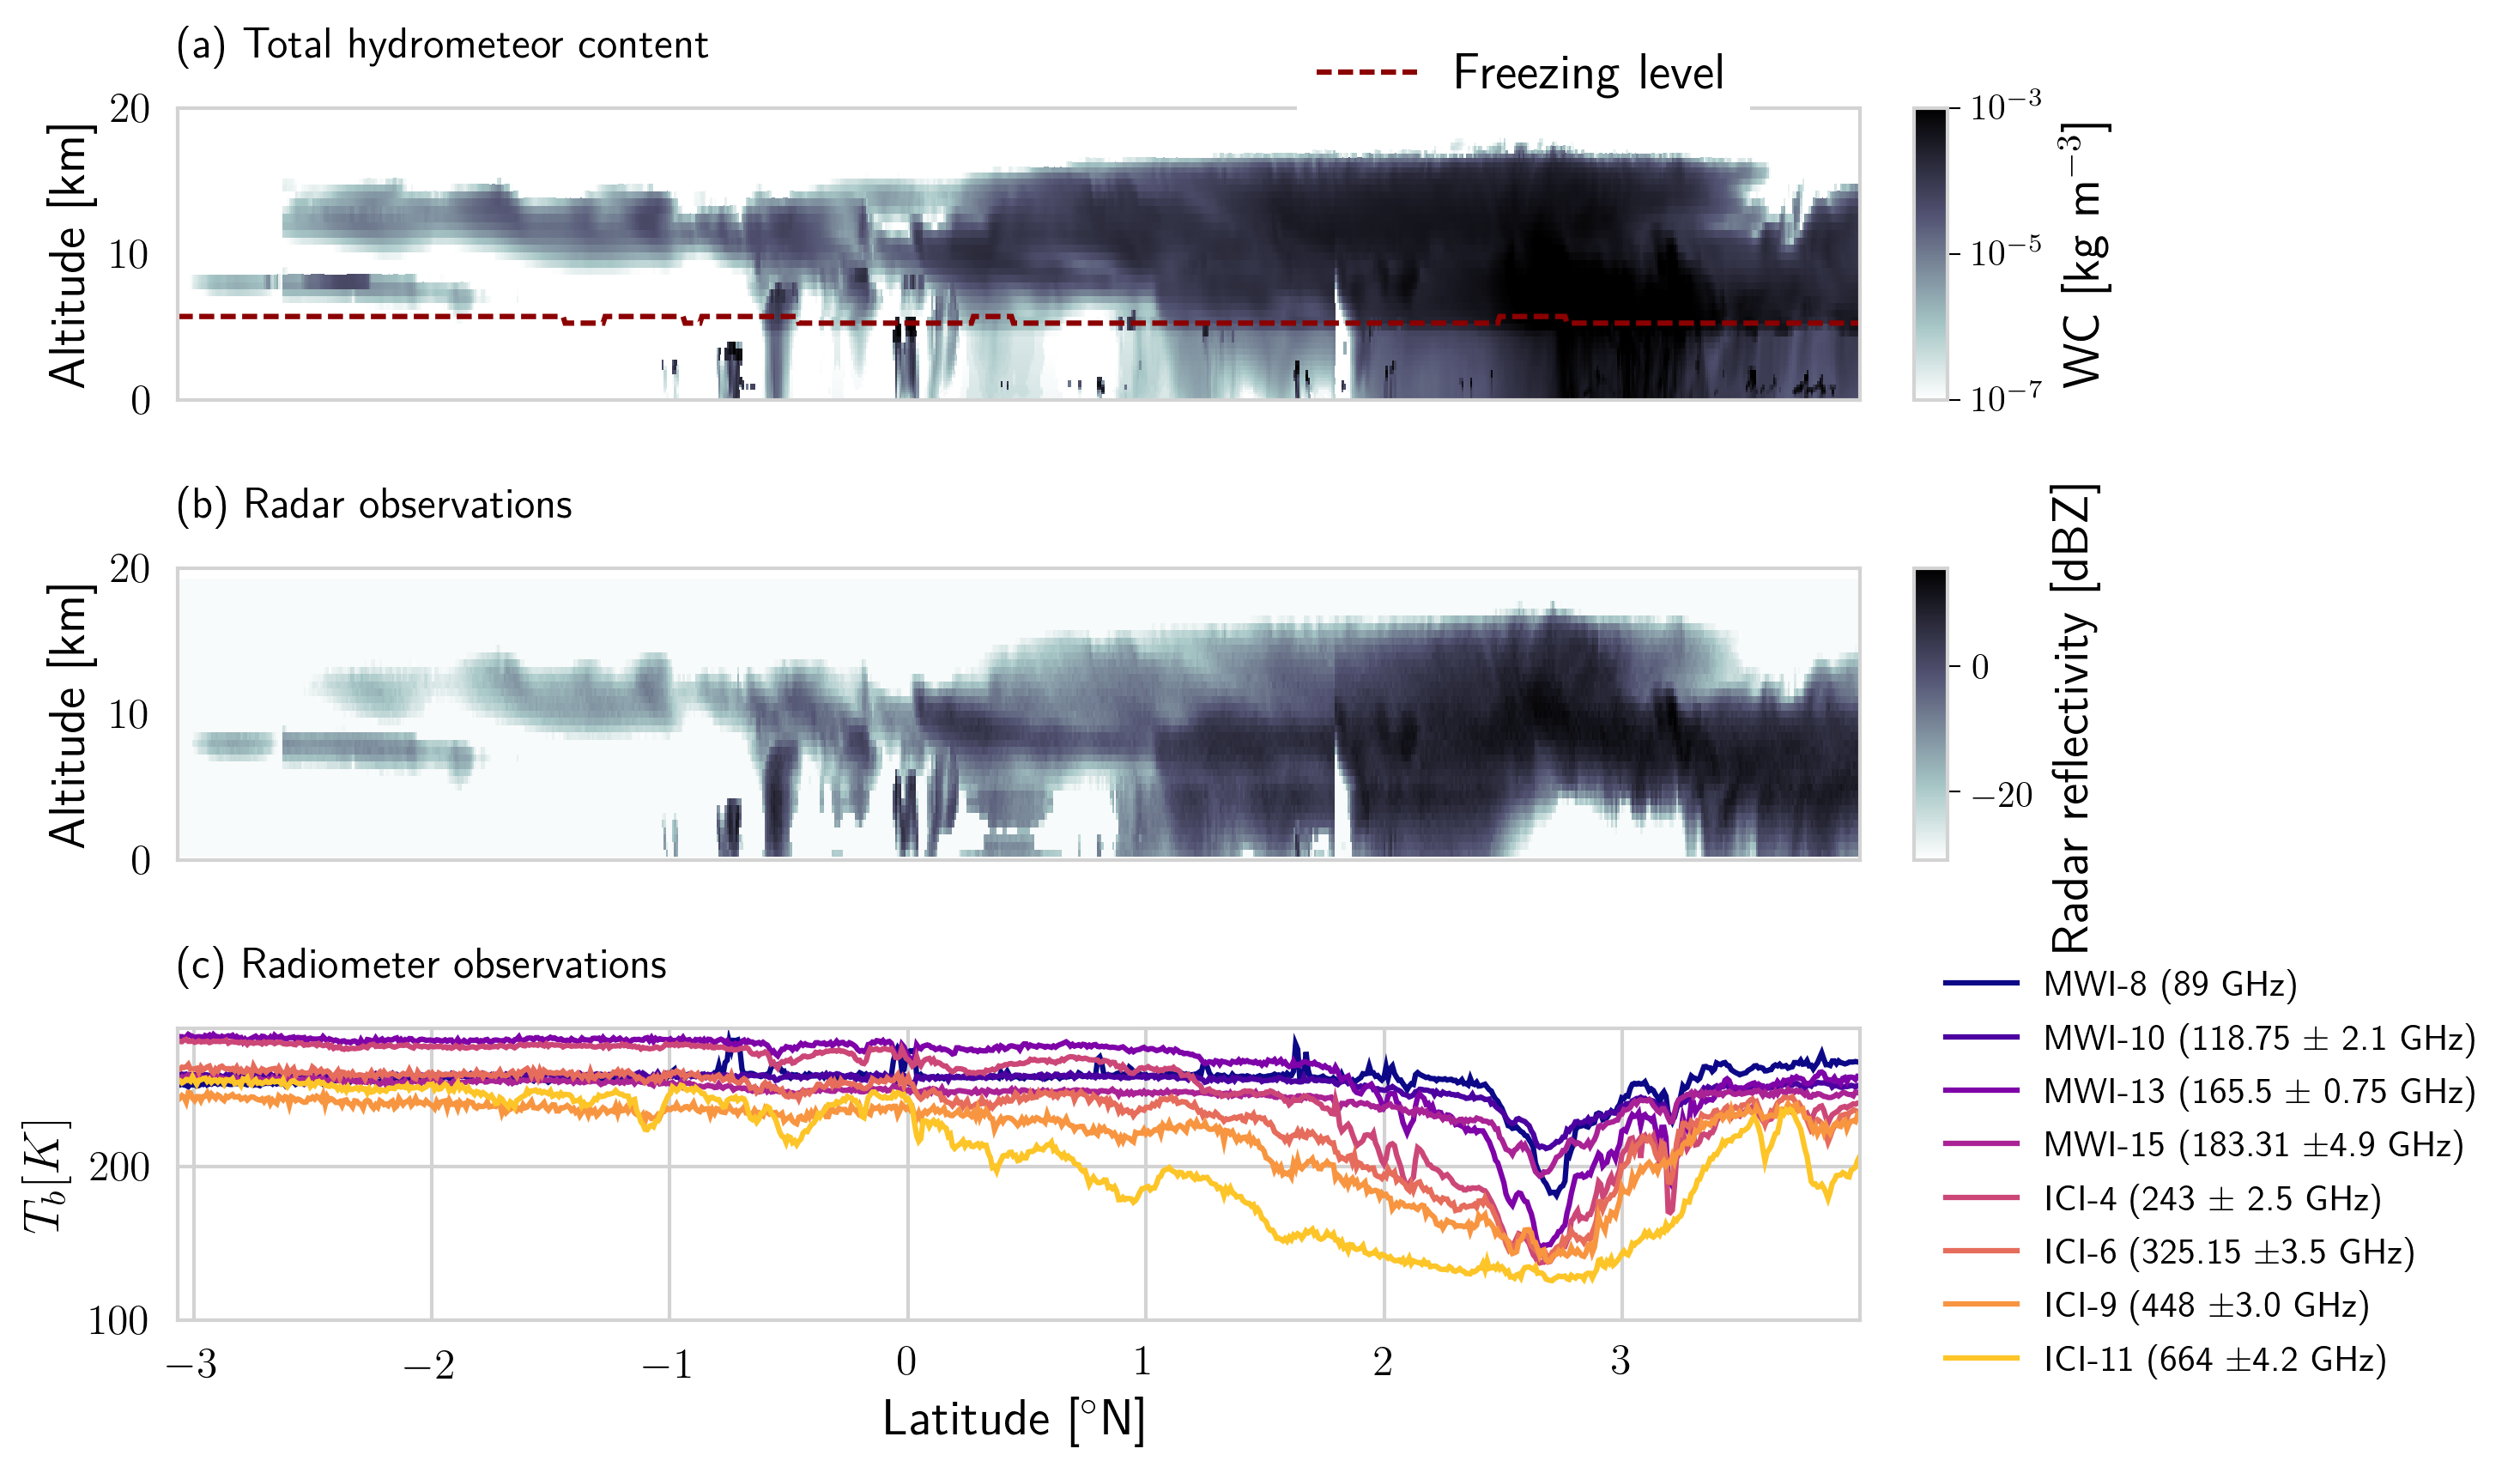
\includegraphics[width = 0.8\textwidth]{../plots/observations_a}
\caption{Total water content (WC) and simulated observations for the first test
  scene. Panel (a) displays the total water content in the scene, i.e. the sum
  of the water content of all hydrometeor species of the GEM model. Panel (b)
  shows the simulated radar reflectivities. Panel (c) displays the simulated
  brightness temperatures for a selection of channels of the MWI and ICI
  radiometers.}
\label{fig:observations_a}
\end{figure}

%Freezing layer has been added to Fig.~5, which now looks as follows:
%
%\begin{figure}
%\centering
%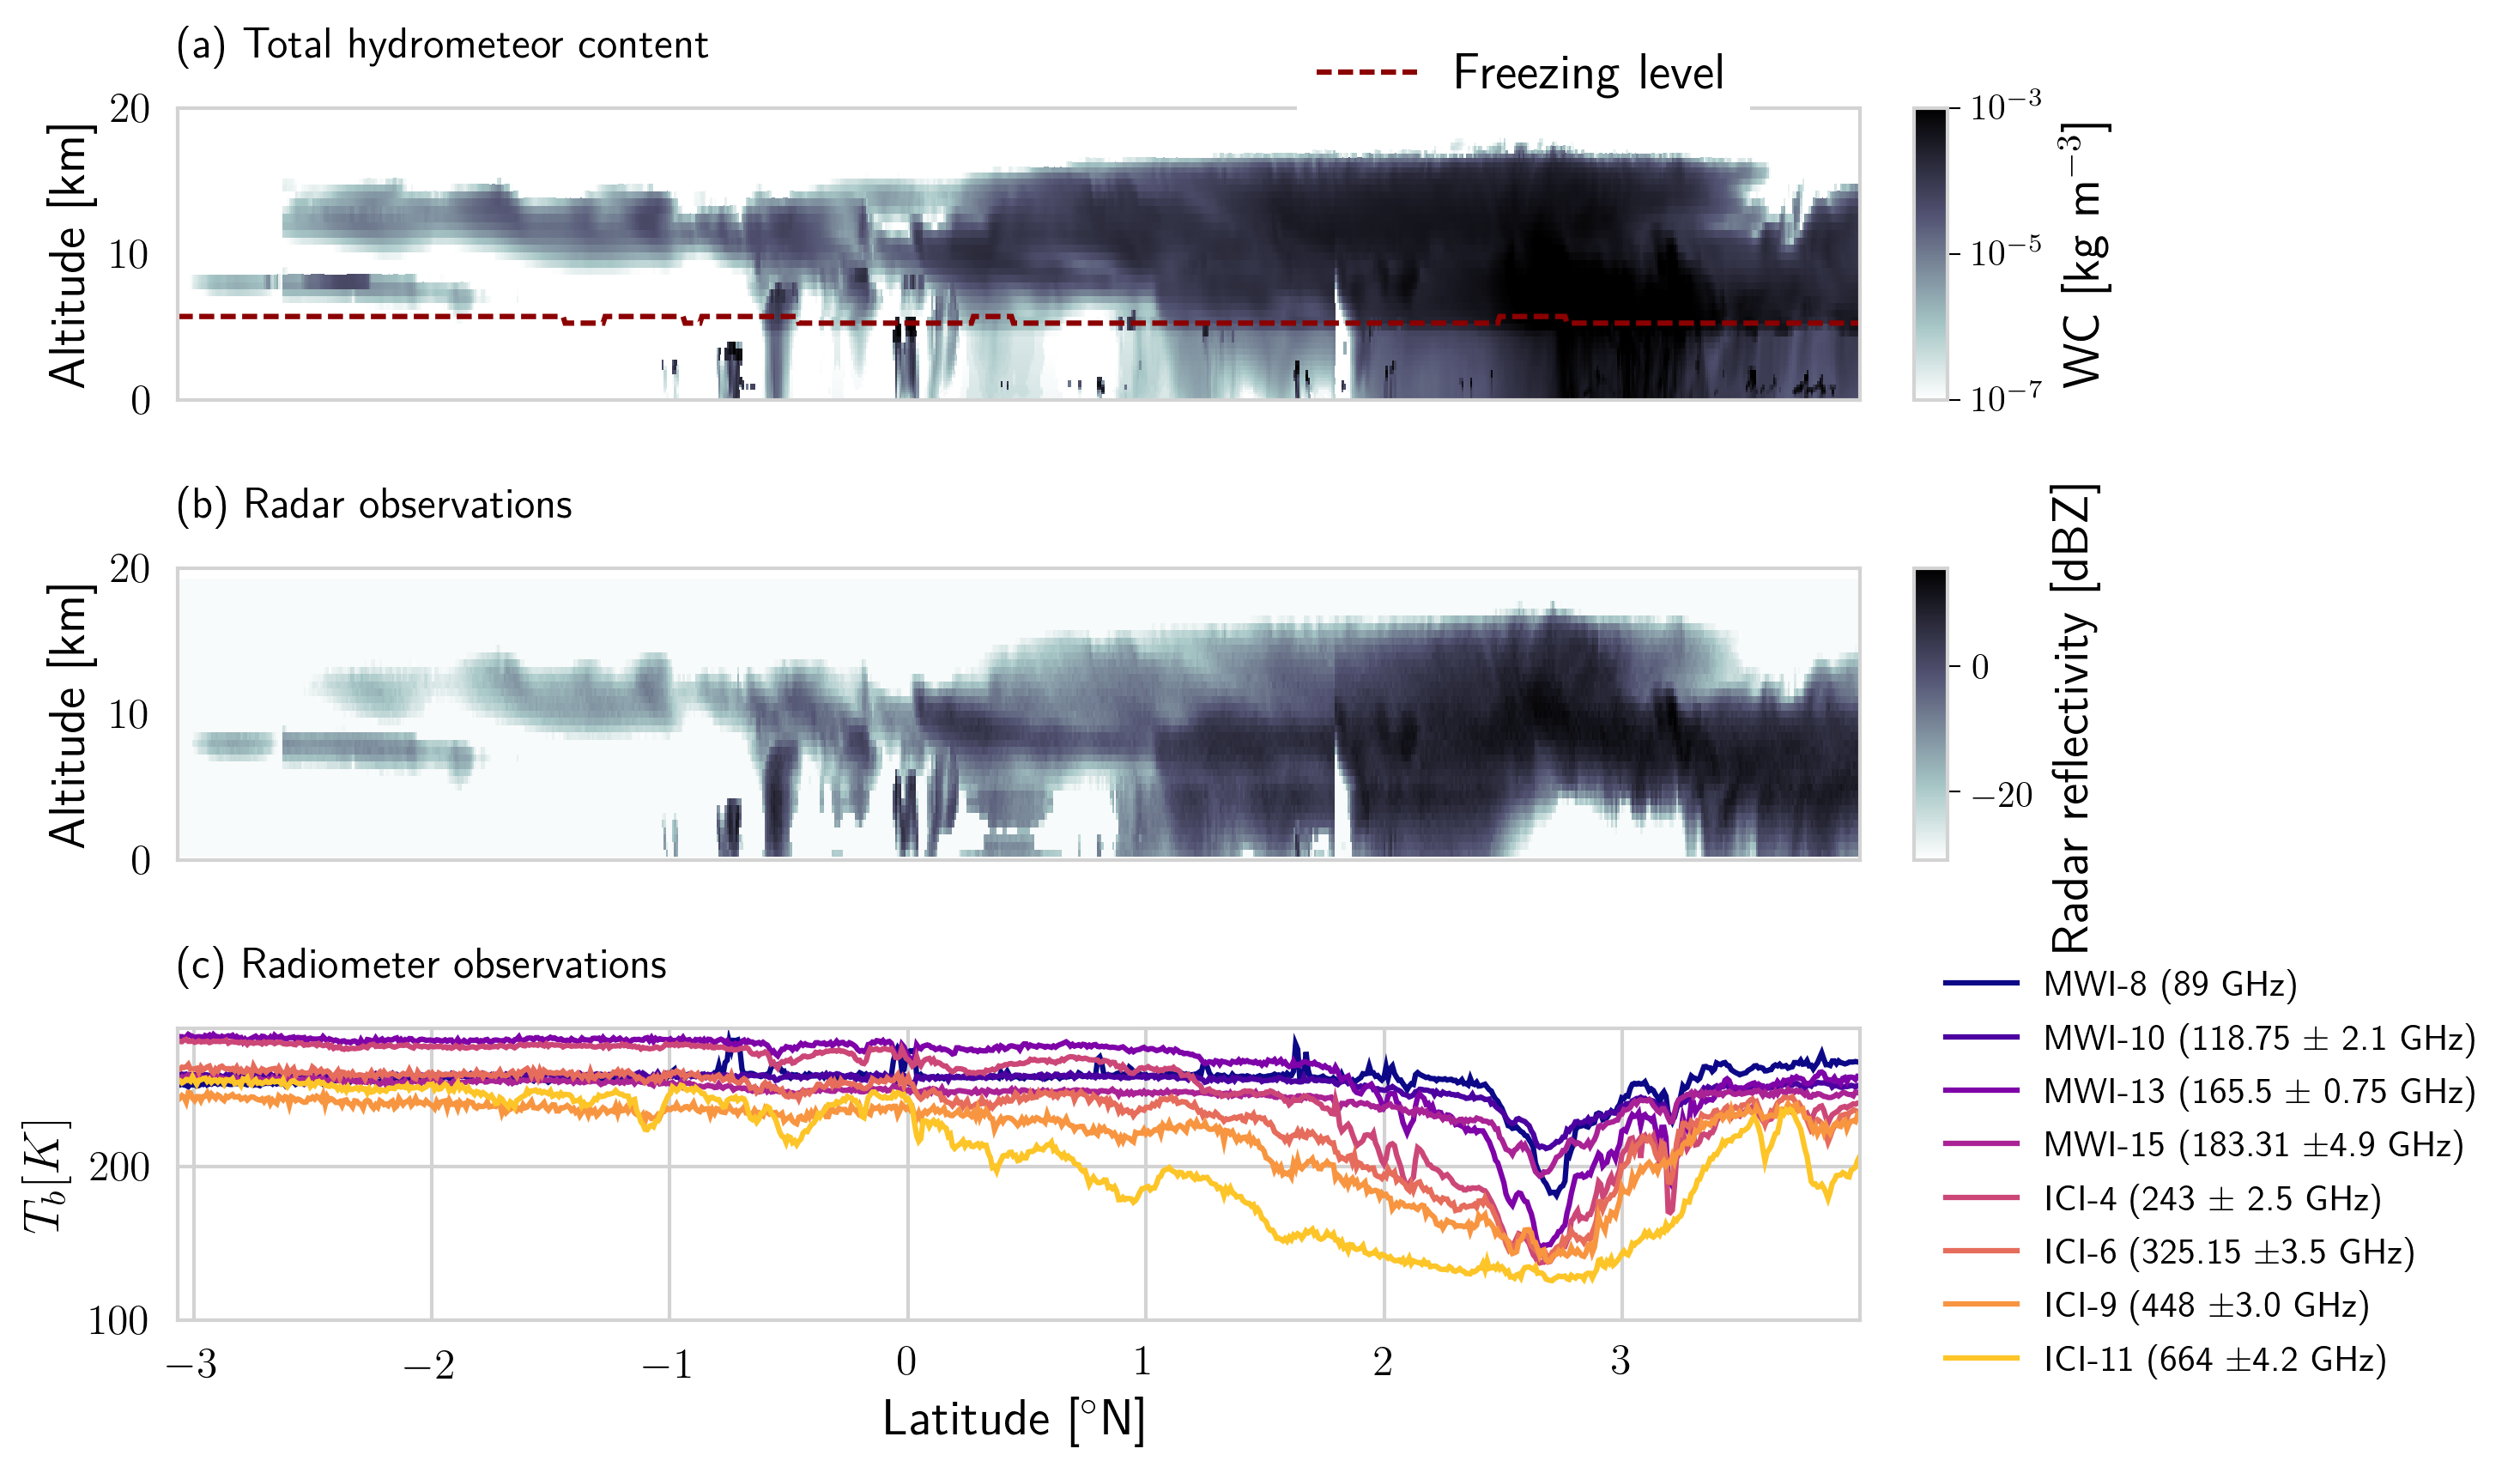
\includegraphics[width = 0.8\textwidth]{../plots/observations_a.png}
%\caption{Total hydrometeor content (HMC) and simulated observations for the first test
%  scene. Panel (a) displays the total hydrometeor content in the scene, i.e. the
%  sum of the mass densities of all hydrometeor species of the GEM model. Panel
%  (b) shows the simulated radar reflectivities. Panel (c) displays the simulated
%  brightness temperatures for a selection of the channels of the MWI and ICI
%  radiometers.}
%\label{fig:observations_a}
%\end{figure}


\subsection*{Reviewer comment 28}
Fig.  6:  It would be nice to see the absolute values of IWP somewhere.  Maybe you could add another time series with IWP as the sum of the different components such that the reader can see where the different categories (cloud, graupel, snow and hail) contribute most?

\subsubsection*{Author response}

We will add absolute IWP and its decomposition into different hydrometeor
classes to Fig. 6.

\subsubsection*{Changes in manuscript}

Total IWP and its decomposition into contributions from different hydrometeor
classes have been added to panel (b) of Fig.~6, which now looks as shown in
Fig.~\ref{fig:results_a}.

\begin{figure}
\centering
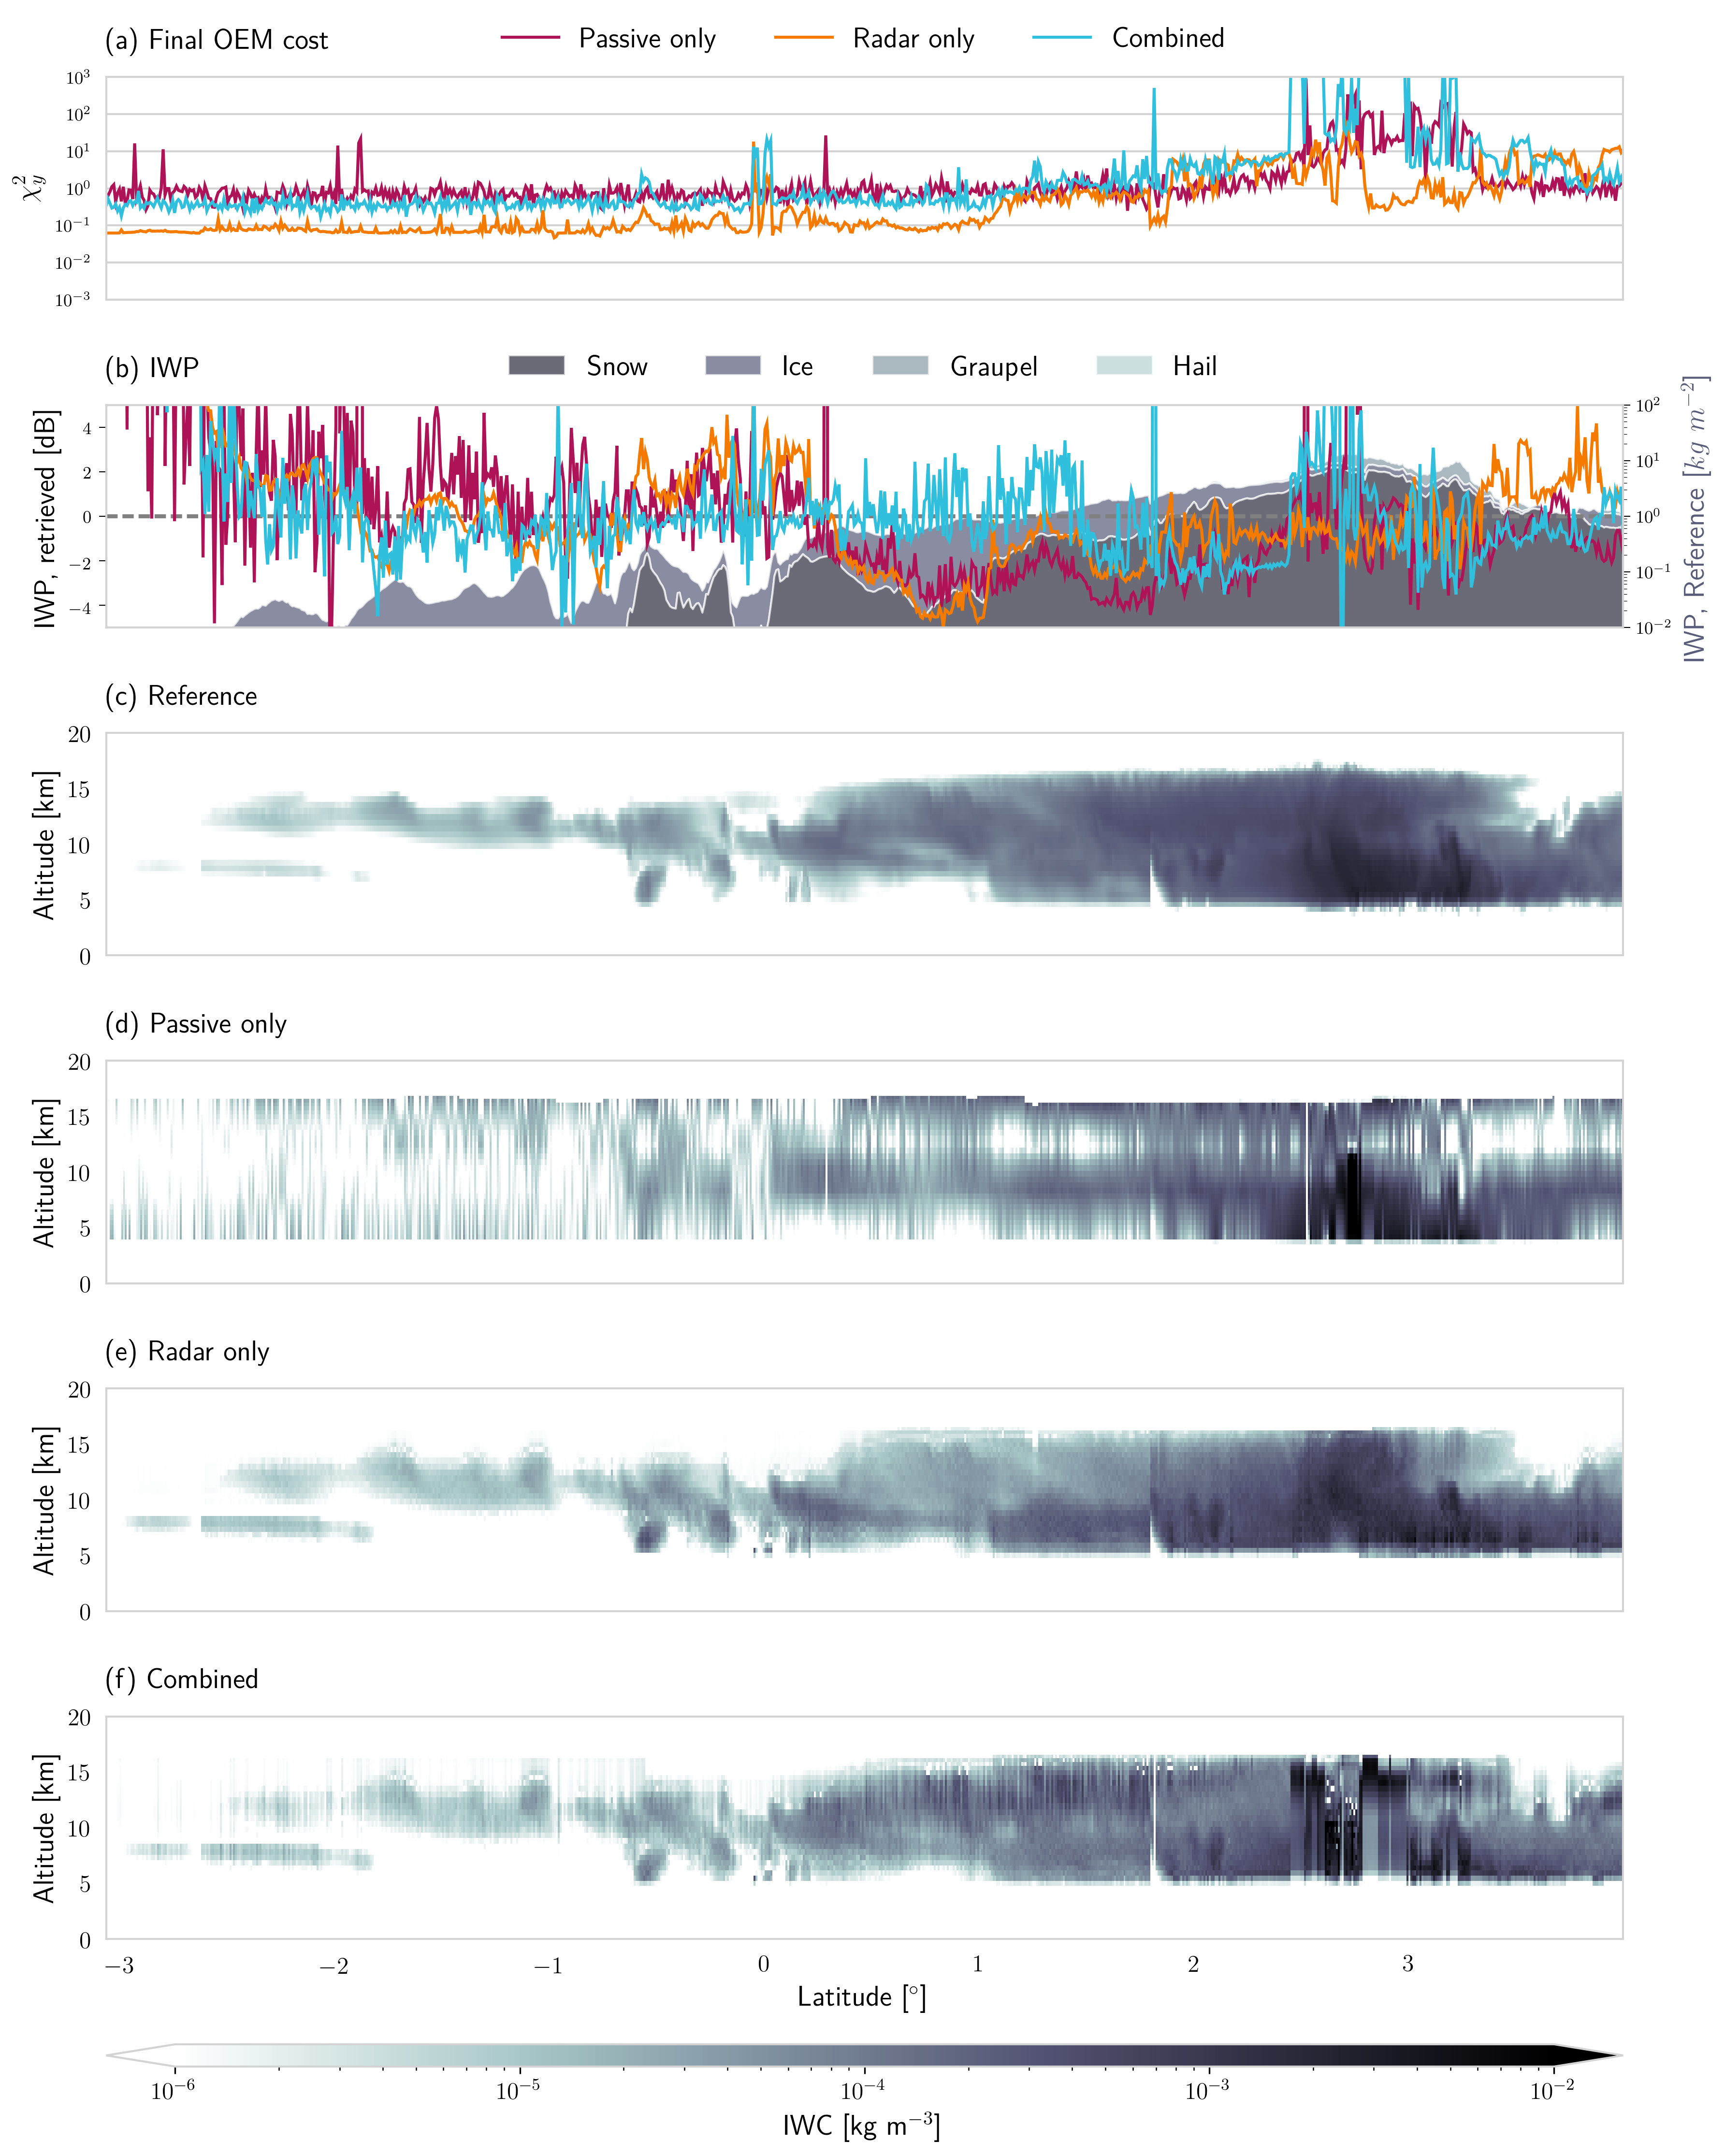
\includegraphics[width = 0.8\textwidth]{../plots/results_a_LargePlateAggregate}
\caption{Results of the ice hydrometeor retrieval for the first test scene using
  the Large Plage Aggregate particle shape. Panel (a) displays the value of the
  $\chi^2_y$ diagnostic normalized by the dimension of the measurement space of
  the corresponding retrieval. Panel (b) displays retrieved IWP in dB relative
  to the reference IWP. Reference IWP and the contributions from different
  hydrometeor classes are displayed by the filled areas in the background. Panel
  (c) shows the reference IWC from the model scene. Panel (d), (e) and (f)
  display the retrieval results for the passive-only, radar-only and combined
  retrieval, respectively.}
\label{fig:results_a}
\end{figure}

%To address the reviewers request the figure will be modified as follows:
%
%\begin{figure}
%\centering
%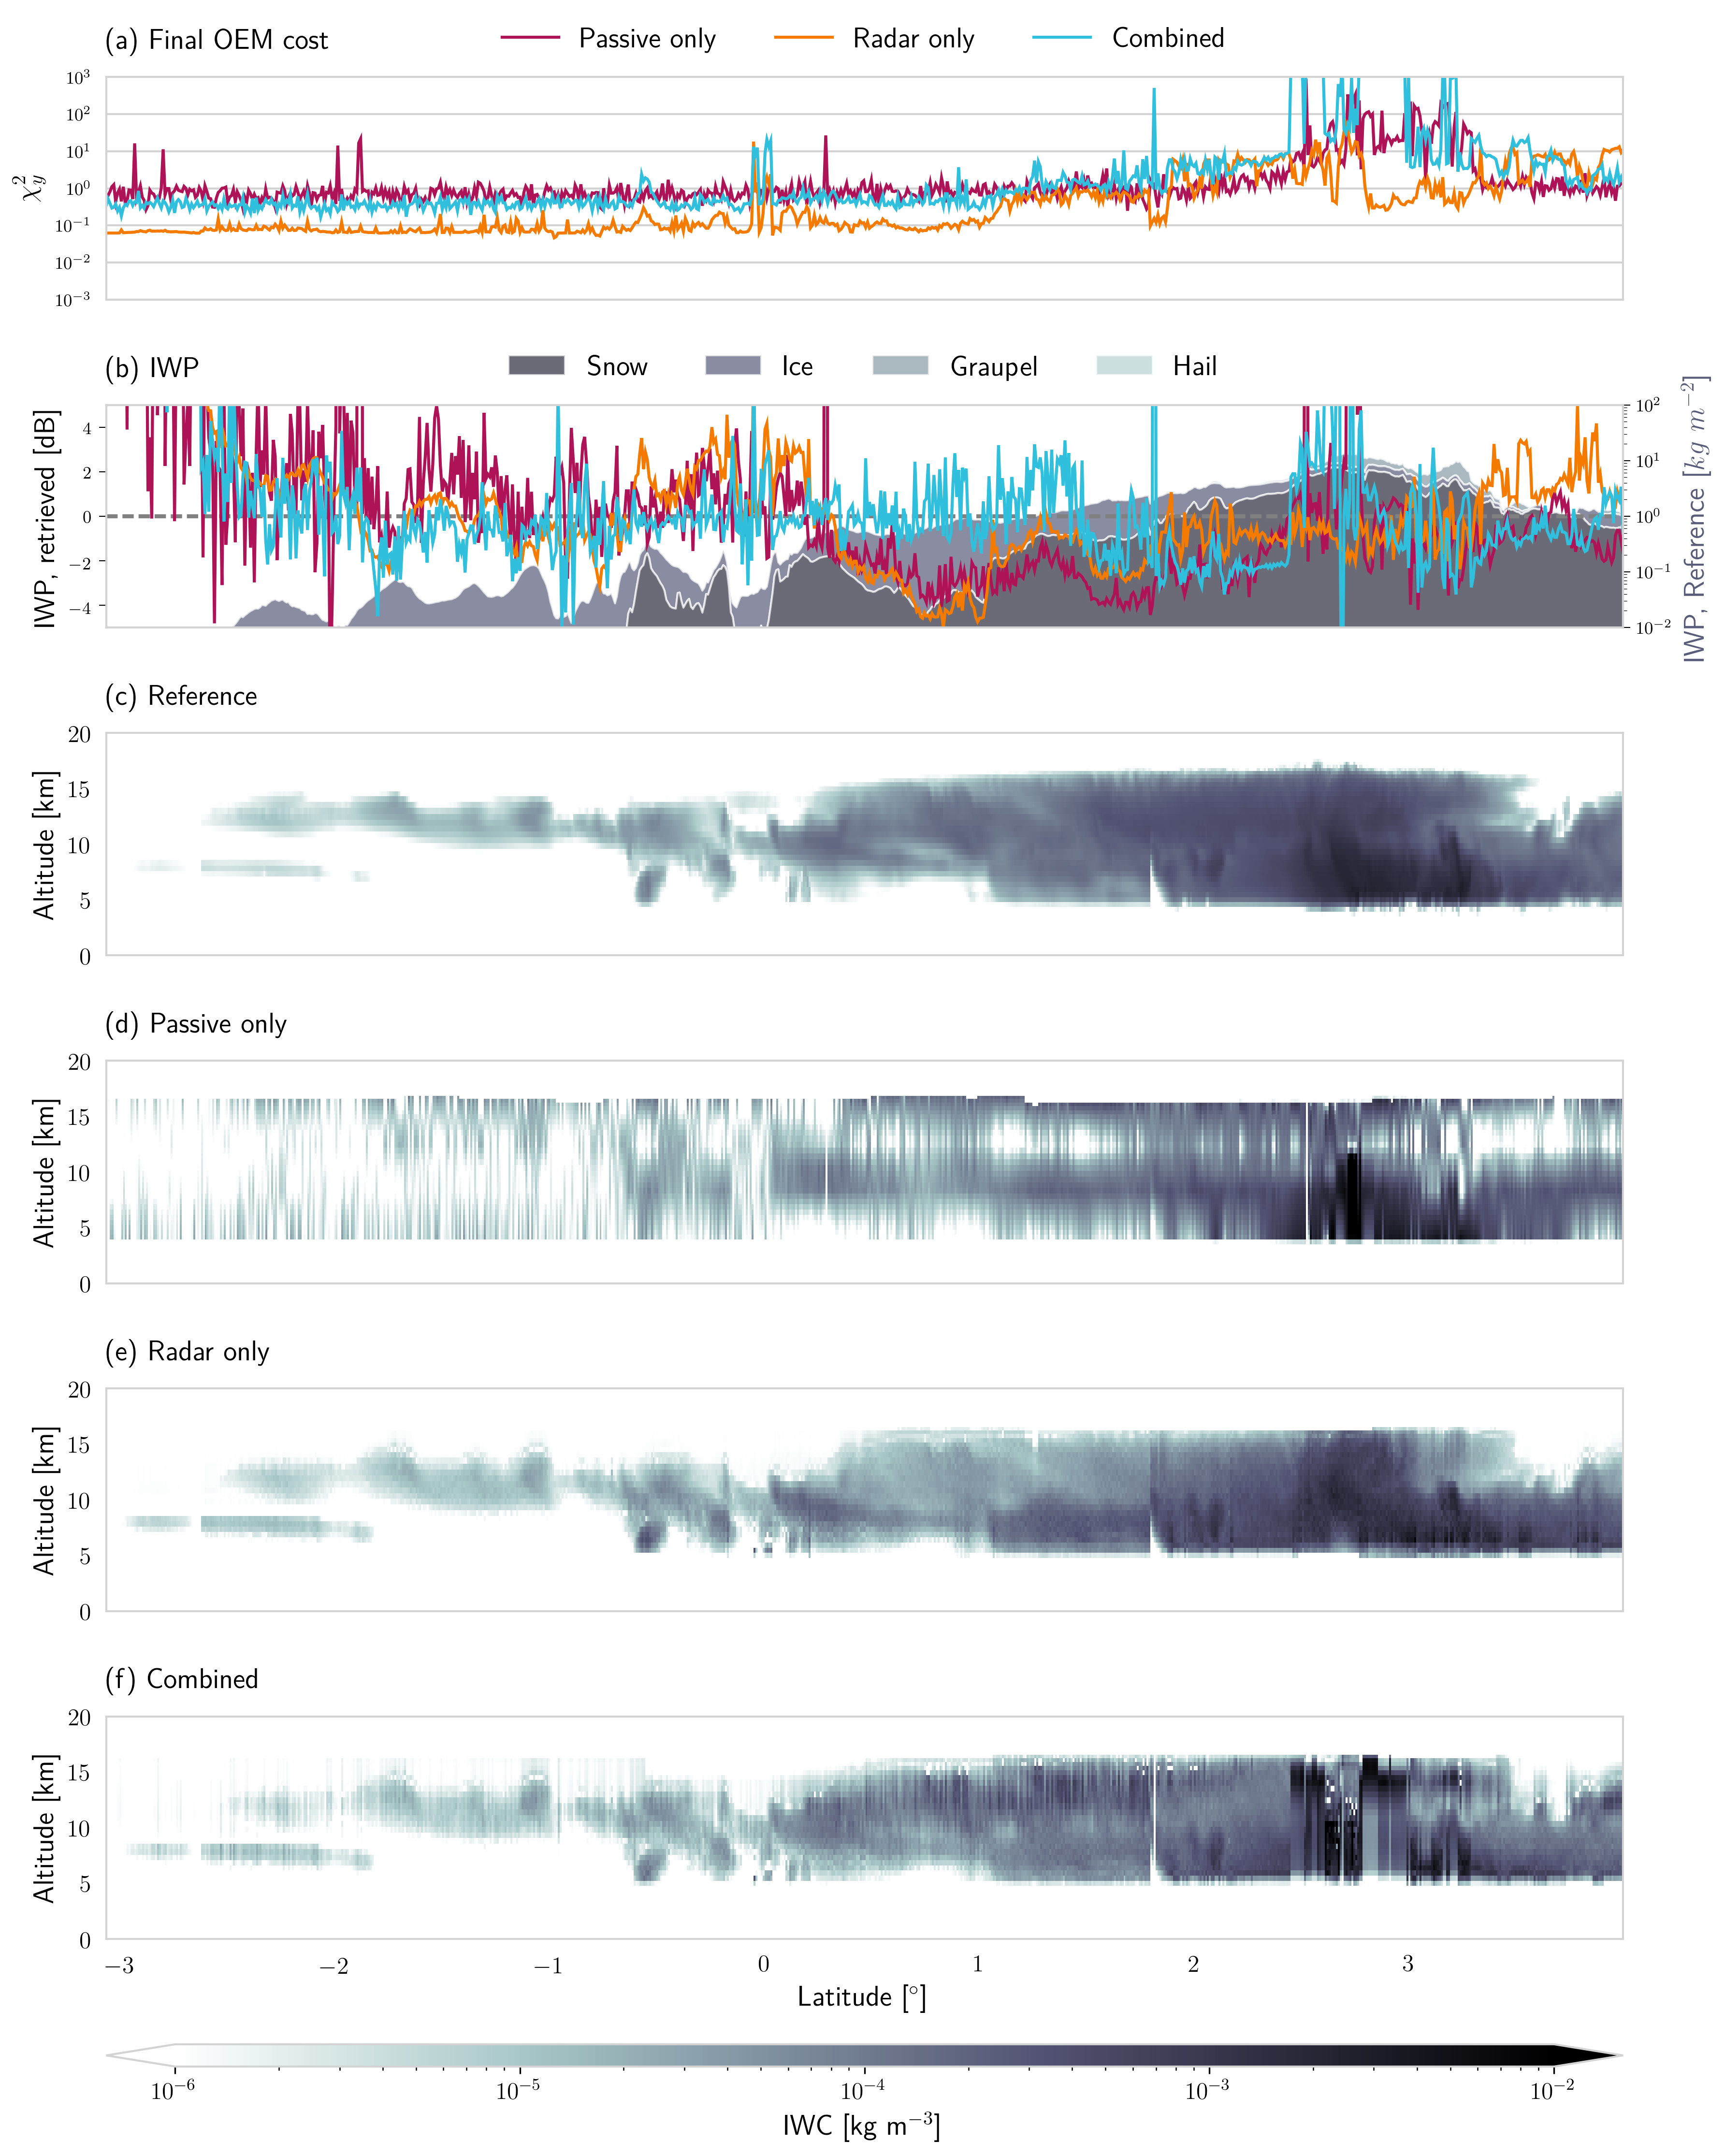
\includegraphics[width = 0.8\textwidth]{../plots/results_a_LargePlateAggregate.png}
%\caption{Results of the ice hydrometeor retrieval for the first test scene.
%  Panel (a) displays the value of the $\chi^2_y$ diagnostic normalized by the
%  dimension of the measurement space of the corresponding retrieval. Panel (b)
%  displays retrieved IWP in dB relative to the reference IWP. Panel (c) shows
%  the reference IWC from the model scene. Panel (d), (e) and (f) display the
%  retrieval results for the passive-only, radar-only and combined retrieval,
%  respectively.}
%\label{fig:results_a}
%\end{figure}


\subsection*{Reviewer comment 29}
Fig. 7: I think it is retrieved vs. truth. The word following is not really
exact. Why not put 7 and 8 together?

\subsubsection*{Author response}

Fig. 7 and 8 have been merged and the caption has been corrected.

\subsubsection*{Changes in manuscript}

C.f. Comments from Referee 1 - Reviewer comment 9.

\subsection*{Reviewer comment 30}
Fig. 9: Could go to the appendix

\subsubsection{Author response}
Fig.~9 has been moved to the appendix.

\subsection*{Reviewer comment 31}
Fig. 10 I only see the caption???

\subsubsection*{Author response}


C.f. Comments from Referee 1 - Reviewer comment 10.

\subsection*{Reviewer comment 32}

Tab. 1. Assumed particle model information for each hydrometeor class given by
GEMmodel. In fact it could be good to combine it

\subsubsection*{Author response}

In order to give a better overview of the particle models that are used
in the retrieval Tab.~4 will be extended in the revised version of the
manuscript.  This, however, would make merging Tab.~1 and 4 slightly confusing
so we decided against the reviewers recommendation.

\subsection*{Reviewer comment 33}

Tab.3 : I would recommend to add a first column with a spelled out name

\subsubsection*{Author response}

We have added the column to the revised version of the manuscript.

\subsubsection*{Changes in manuscript}

The proposed column has been added to the table which now looks as is shown
in Tab.~\ref{tab:a_priori}.

\begin{table}[h!]
\caption{A priori uncertainties and correlation
 lengths used in the retrieval.}
 \centering
\label{tab:a_priori}
  \begin{adjustbox}{max width=\textwidth}
    \begin{tabular}{ll|cc|cc|}
      \multicolumn{2}{c|}{Retrieval target}  & \multicolumn{2}{c|}{Combined / Radar-only} & \multicolumn{2}{c}{Passive-only}\\
      Name & Retrieved quantity &  $\sigma_q$ & $l_q$ [km] & $\sigma_q$ & $l_q$ [km]\\
    \hline
Ice, $N_0^*$ & $\log_{10}(N_{0, \text{Ice}}^*)$ & $2$ & $2$ & $2$ &$5$ \\
Ice, $D_m$ &   $\text{Ice }D_{m, \text{Ice}}$   & $300\ \unit{\mu m}$  & $2$ & $300\ \unit{\mu m}$          & $5$ \\
Rain, $N_0^*$ &    $\log_{10}(\text{Rain } N_{0}^*)$ & $2$ & $2$ & $2$ &$5$ \\
Rain, $D_m$ &  $D_{m, \text{Rain}}$   & $300\ \unit{\mu m}$  & $2$ & $300\ \unit{\mu m}$          & $5$ \\
Relative humidity (RH) & $\text{arctanh}(\frac{2 \cdot \text{RH}}{1.2} - 1.0)$ & $0.5^{*}$ & $2^{*}$ & $0.5$ & $2$ \\
Cloud liquid water content (CLWC) & $\log_{10}(\text{CLWC}) $ & $1^{*}$ & $2^{*}$  & $1$ & $2$ \\
\multicolumn{6}{l}{$^*$: Not retrieved in radar-only retrieval}
    \end{tabular}
    \end{adjustbox}
\end{table}
\section{Grammar, typos and reformulations}

The authors would like to thank the reviewer for the additional comments, all of
which will be incorporated into the revised manuscript.
